
\chapter{Models AP in Purkinje fibre}
\label{chap:models-ap-purkinje}


Purkinje fibre cell is a cardiac non-pacemaker cell. Its AP is
self-oscillatory, with a sharp upstroke that overshoots and return to
a prolonged plateau (300-400 ms), compared to 3ms in the squid axon,
before recovering. Also, Purkinje fibre lacks T-tubule, and has two types of SR:
junctional SR and corbular (nonjunctional) SR. Corbular SR is directly under the
surface membrane, with 25\% by volume of myofibrils surrounded by the corbular
SR. The mechanism of ECC in Purkinje fibre is not well understood, though the
role of corbular SR is getting more important from recent studies
\citep{boyden2000}.

The size of canine Purkinje cells is: width (25-30$\mum$), length
(157-314$\mum$) \citep{wier2000}. The model for Purkinje fibre AP first done by
Noble (1962) with 3 ionic currents (read sect.~\ref{sec:noble-model}). Later
experimental data shown multiple slow components in ionic
current~\citep{noble1968krp,noble1969omc}, then McAllister-Noble-Tsien model
was proposed in 1975 (sect.~\ref{sec:macall-noble-tsien}) with 9 ionic currents.

The first studies of $[\Ca]_i$ transient in Purkinje fibers were done by Wier et
al. \citep{wier1980, wier1982} using bioluminescent protein aequorin
(Sect.\ref{sec:aequorin}).
The resting potential was detected in the range -70mV to -85mV; and action potential
(AP) showed amplitude between 100mV to +130mV. The AP duration (APD) at stimulus
interval of 2sec (i.e. 0.5Hz) is about 500-900ms, Fig.\ref{fig:Aequorin_L1L2}.
Peak tension was reached 140ms after the V-clamp initiation, then relaxation
occured over the next 400ms \citep{wier1982}.


\section{Noble model (Purkinje fibre) (1962)}
\label{sec:noble-model}


Since the milestone model for the squid giant axon, there were other
efforts to create model for other cell types. For Purkinje fibre cell
of the heart, the AP has a sharp spike in the early AP, and a long
plateau (300-400ms) compared to that of nerve cell (3ms), as shown in
Fig.~\ref{fig:AP_compare}. In an effort to create a whole-cell model
for the Purkinje fibre, Noble applied the Hodgkin-Huxley model and
modified it~\citep{noble1962mhh}.

% To model this, in
% 1962, Noble made a modification to Hodgkin-Huxley model (built for
% nerve cell).
% \textcolor{red}{Noble model is still a reduction to HH model} as only
% Na current and K current was taken into account, i.e. $I_L$ was
% neglected.

\subsection{Hypothesis analysis}
\label{sec:quant-analys-1}

\begin{figure}[hbt]
  \centerline{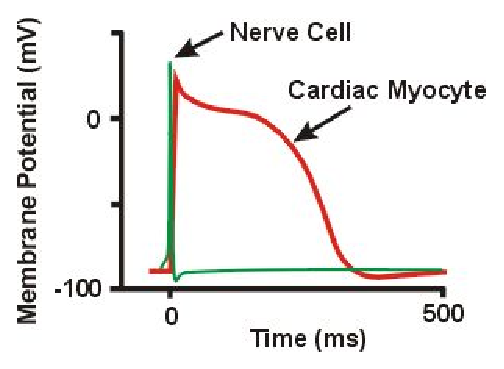
\includegraphics[height=3cm,
    angle=0]{./images/action_potentials_compare.eps}}
\caption{AP of nerve cell and non-pacemaker cardiac cell}
\label{fig:AP_compare}
\end{figure}

\begin{figure}[!hbt]
  \centerline{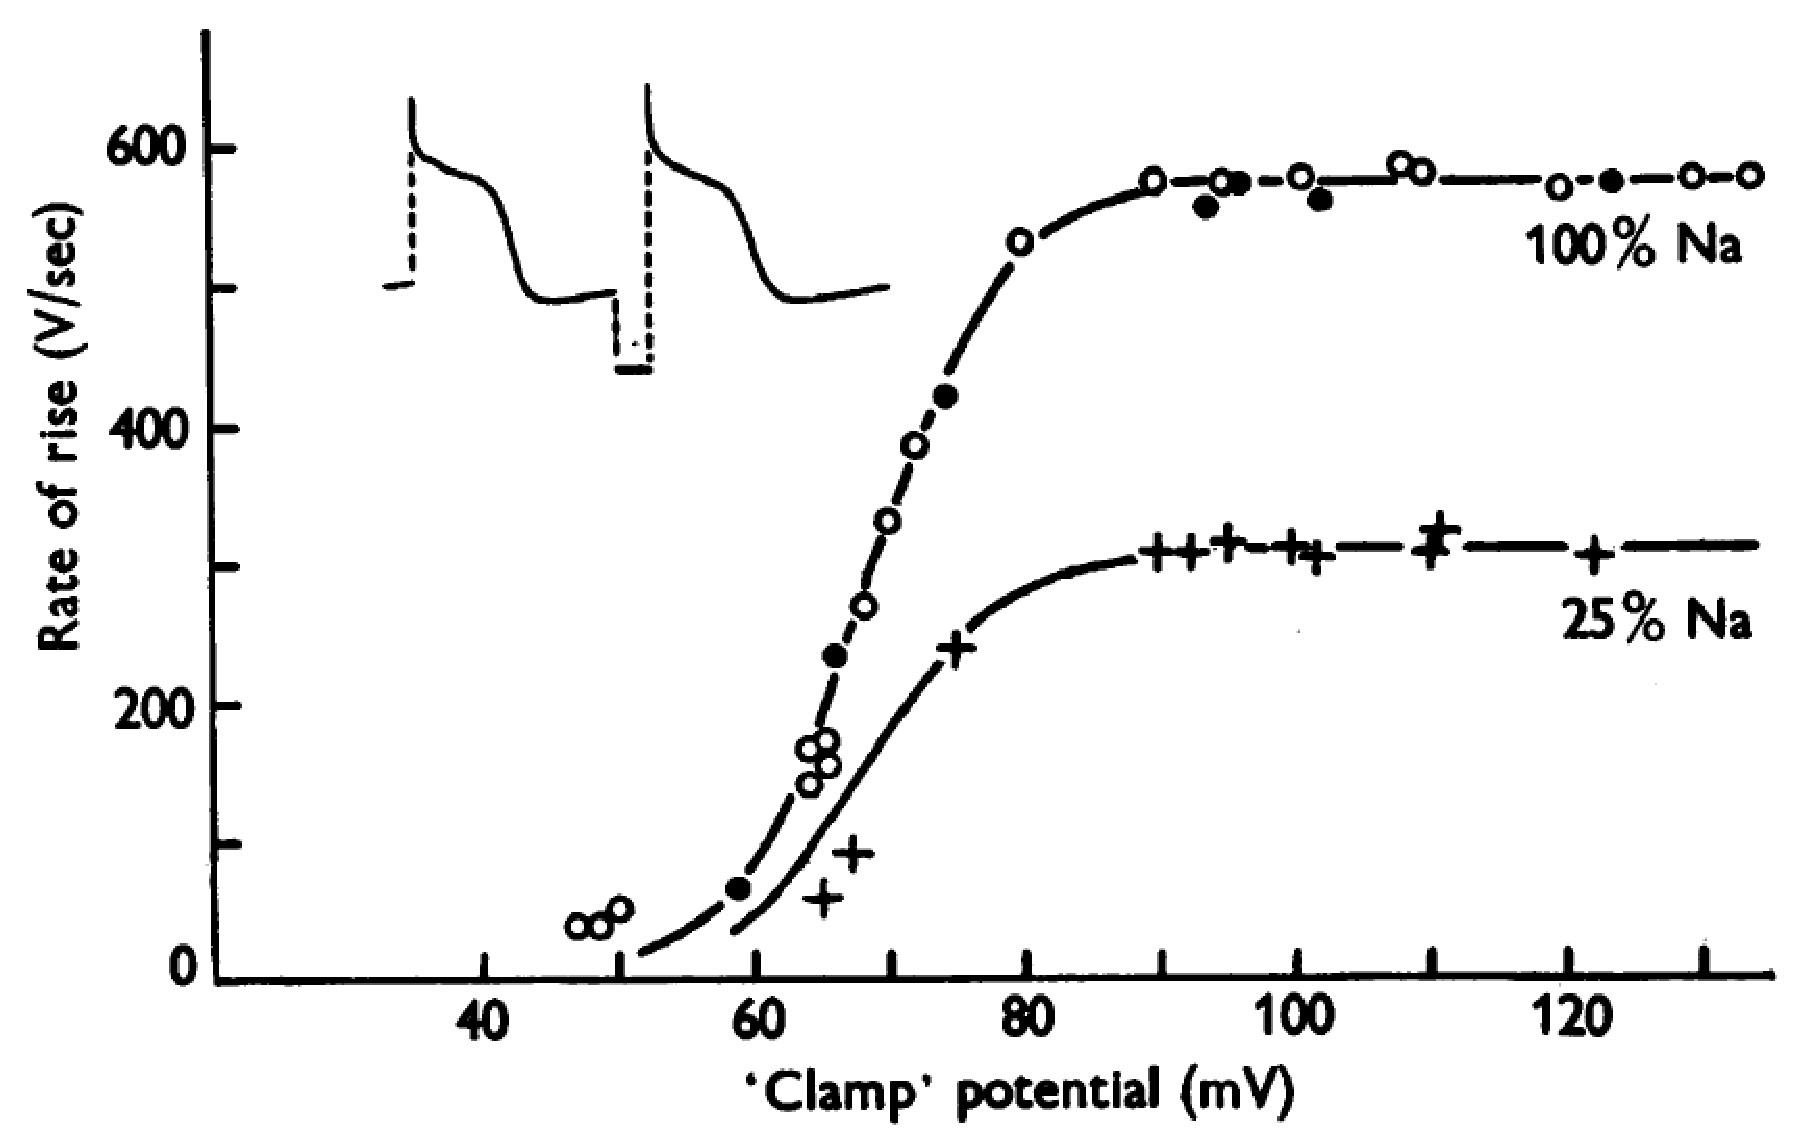
\includegraphics[height=4.5cm]{./images/clamped_potential_Na.eps}}
  \caption{The clamped potential vs. maximum rate of rise of AP, under
    two experiment conditions of [Na] in Tyrode solution}
  \label{fig:clamped_potential}
\end{figure}

\begin{framed}

At that time, accurate measurement of $I_\na$ in Purkinje fiber was impossible
as the time course of the current is too fast to allow adequate voltage clamping
(using high-resistance micro-electrodes) to be in control. Thus, Weidmann
\citep{weidmann1955cmp} developed a method for determining $h$ kinetics without
using full voltage-clamp technique and found that $h$ kinetics strongly resemble
those for nerve, although the $h_\infty(V_m)$ curve is steeper. Another solution
is to measure at low temparature (8$^\circ$C) which can slow the time course by
a factor of about 30x \citep{dudel1970}. However, converting to the value in 
room temperature (37$^\circ$C) using Q10 is not straightforward. So, many
assumed that sodium conductance has a similar behavior to that of nerve cell, as
shown in Fig.~\ref{fig:clamped_potential} and Fig.~\ref{fig:Purkinjie_conduct}.
\end{framed}

\begin{figure}[hbt]
  \centerline{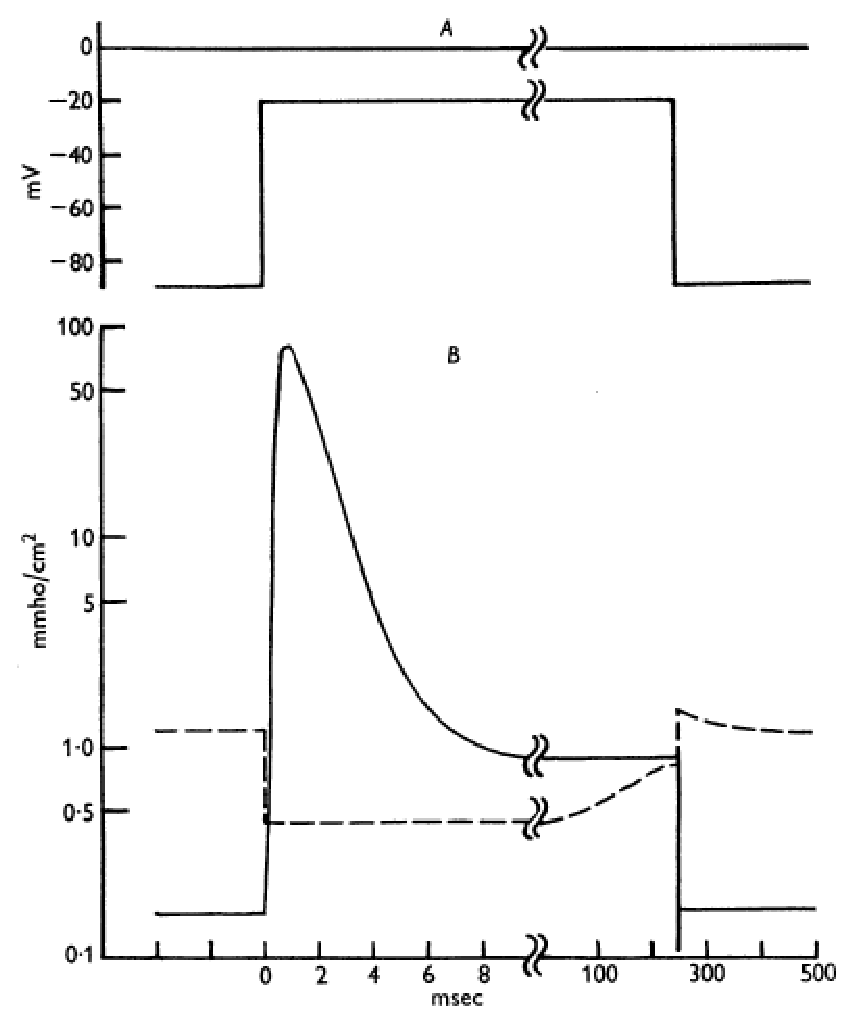
\includegraphics[height=6cm]{./images/Purkinjie_conductance.eps}}
  \caption{(A) Membrane potential $V_m$ (holding: -90, step: -20mV)
    (B) The change in ionic conductance of $\Na$ (continuous curve) and $\K$
    (interrupted curve) on a log. scale (unit: mmho/cm$^2$). NOTE: the time
    scale change after 9ms}
  \label{fig:Purkinjie_conduct}
\end{figure}


In squid axon, the Na conductance follow a biphasic manner with an S-shape
increase (activation) and an exponential decrease (inactivation). The I-V curve
for $\Na$ current in Purkinje fiber is steeper than that for squid nerve.
Nevertheless, Noble hypothesized the same kinetics, by reasoning that the
steepness was due to the difference in experimental technique. Noble thus used
Hodgkin-Huxley formula for Na current\footnote{ However, at that time, there was
still no quantitative way to predict the affect of \ce{Na+} on the rate of AP
rising}. 

Given the difference in APD, the plateau in the AP of Purkinje fibre was
accounted by $\Na$ channel (at this time the role of $\Ca$ was not confirmed and
ignored). Noble assume that the inward sodium current take the dual role:
generating the upstroke of AP ({\it pacemaker current}) and maintain the prolong
plateau in the AP. That's why a small quantity conductance $g_i$ was added to
$g_{Na}$, eq.~\eqref{eq:607}. (\textcolor{red}{This hypothesis is incorrect, as
we will learn that it is Ca current that prolongs the AP plateau}).

\begin{figure}[hbt]
  \centerline{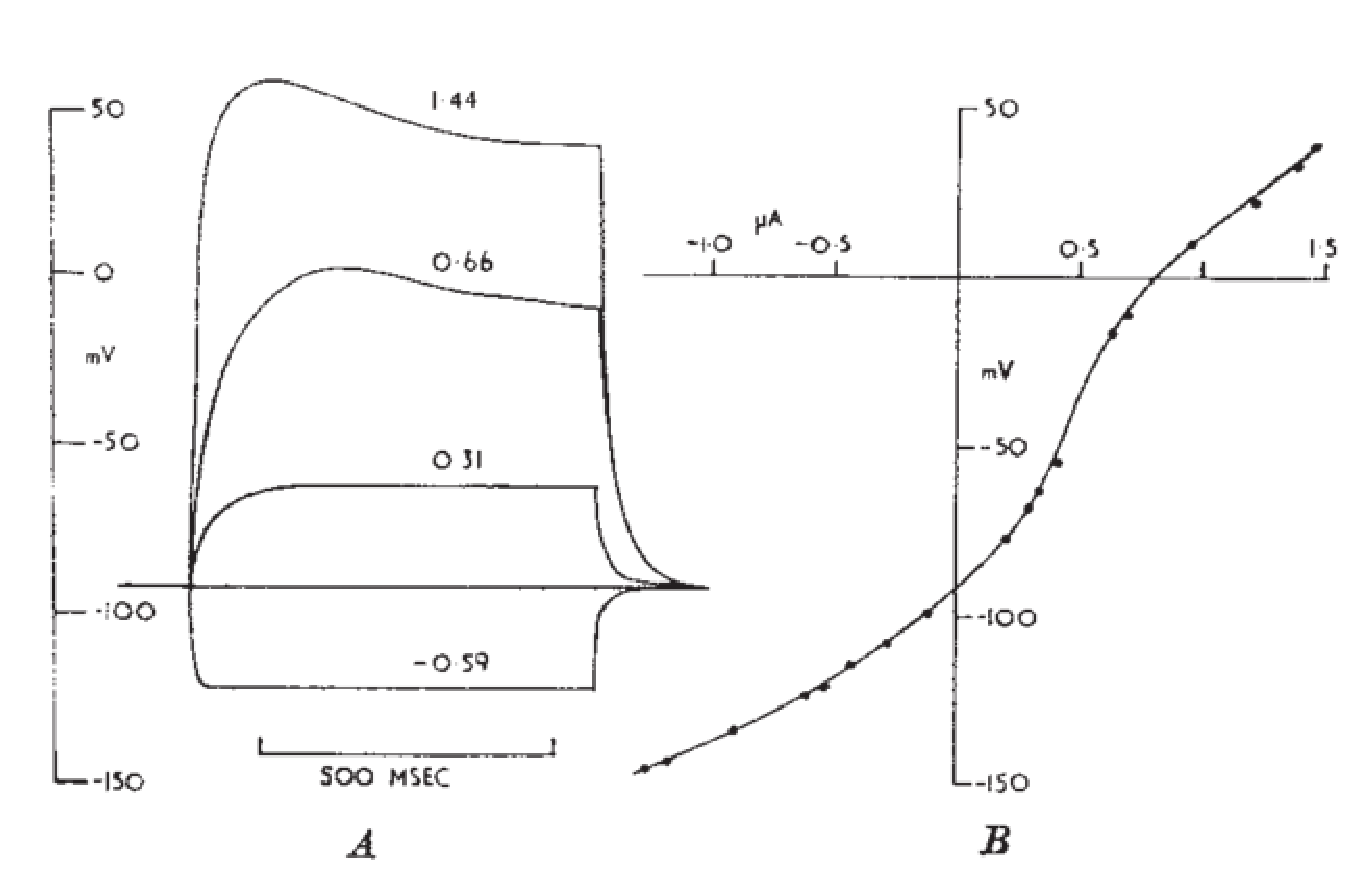
\includegraphics[height=4cm,
    angle=0]{./images/Hutter1960_Kcurrent.eps}; 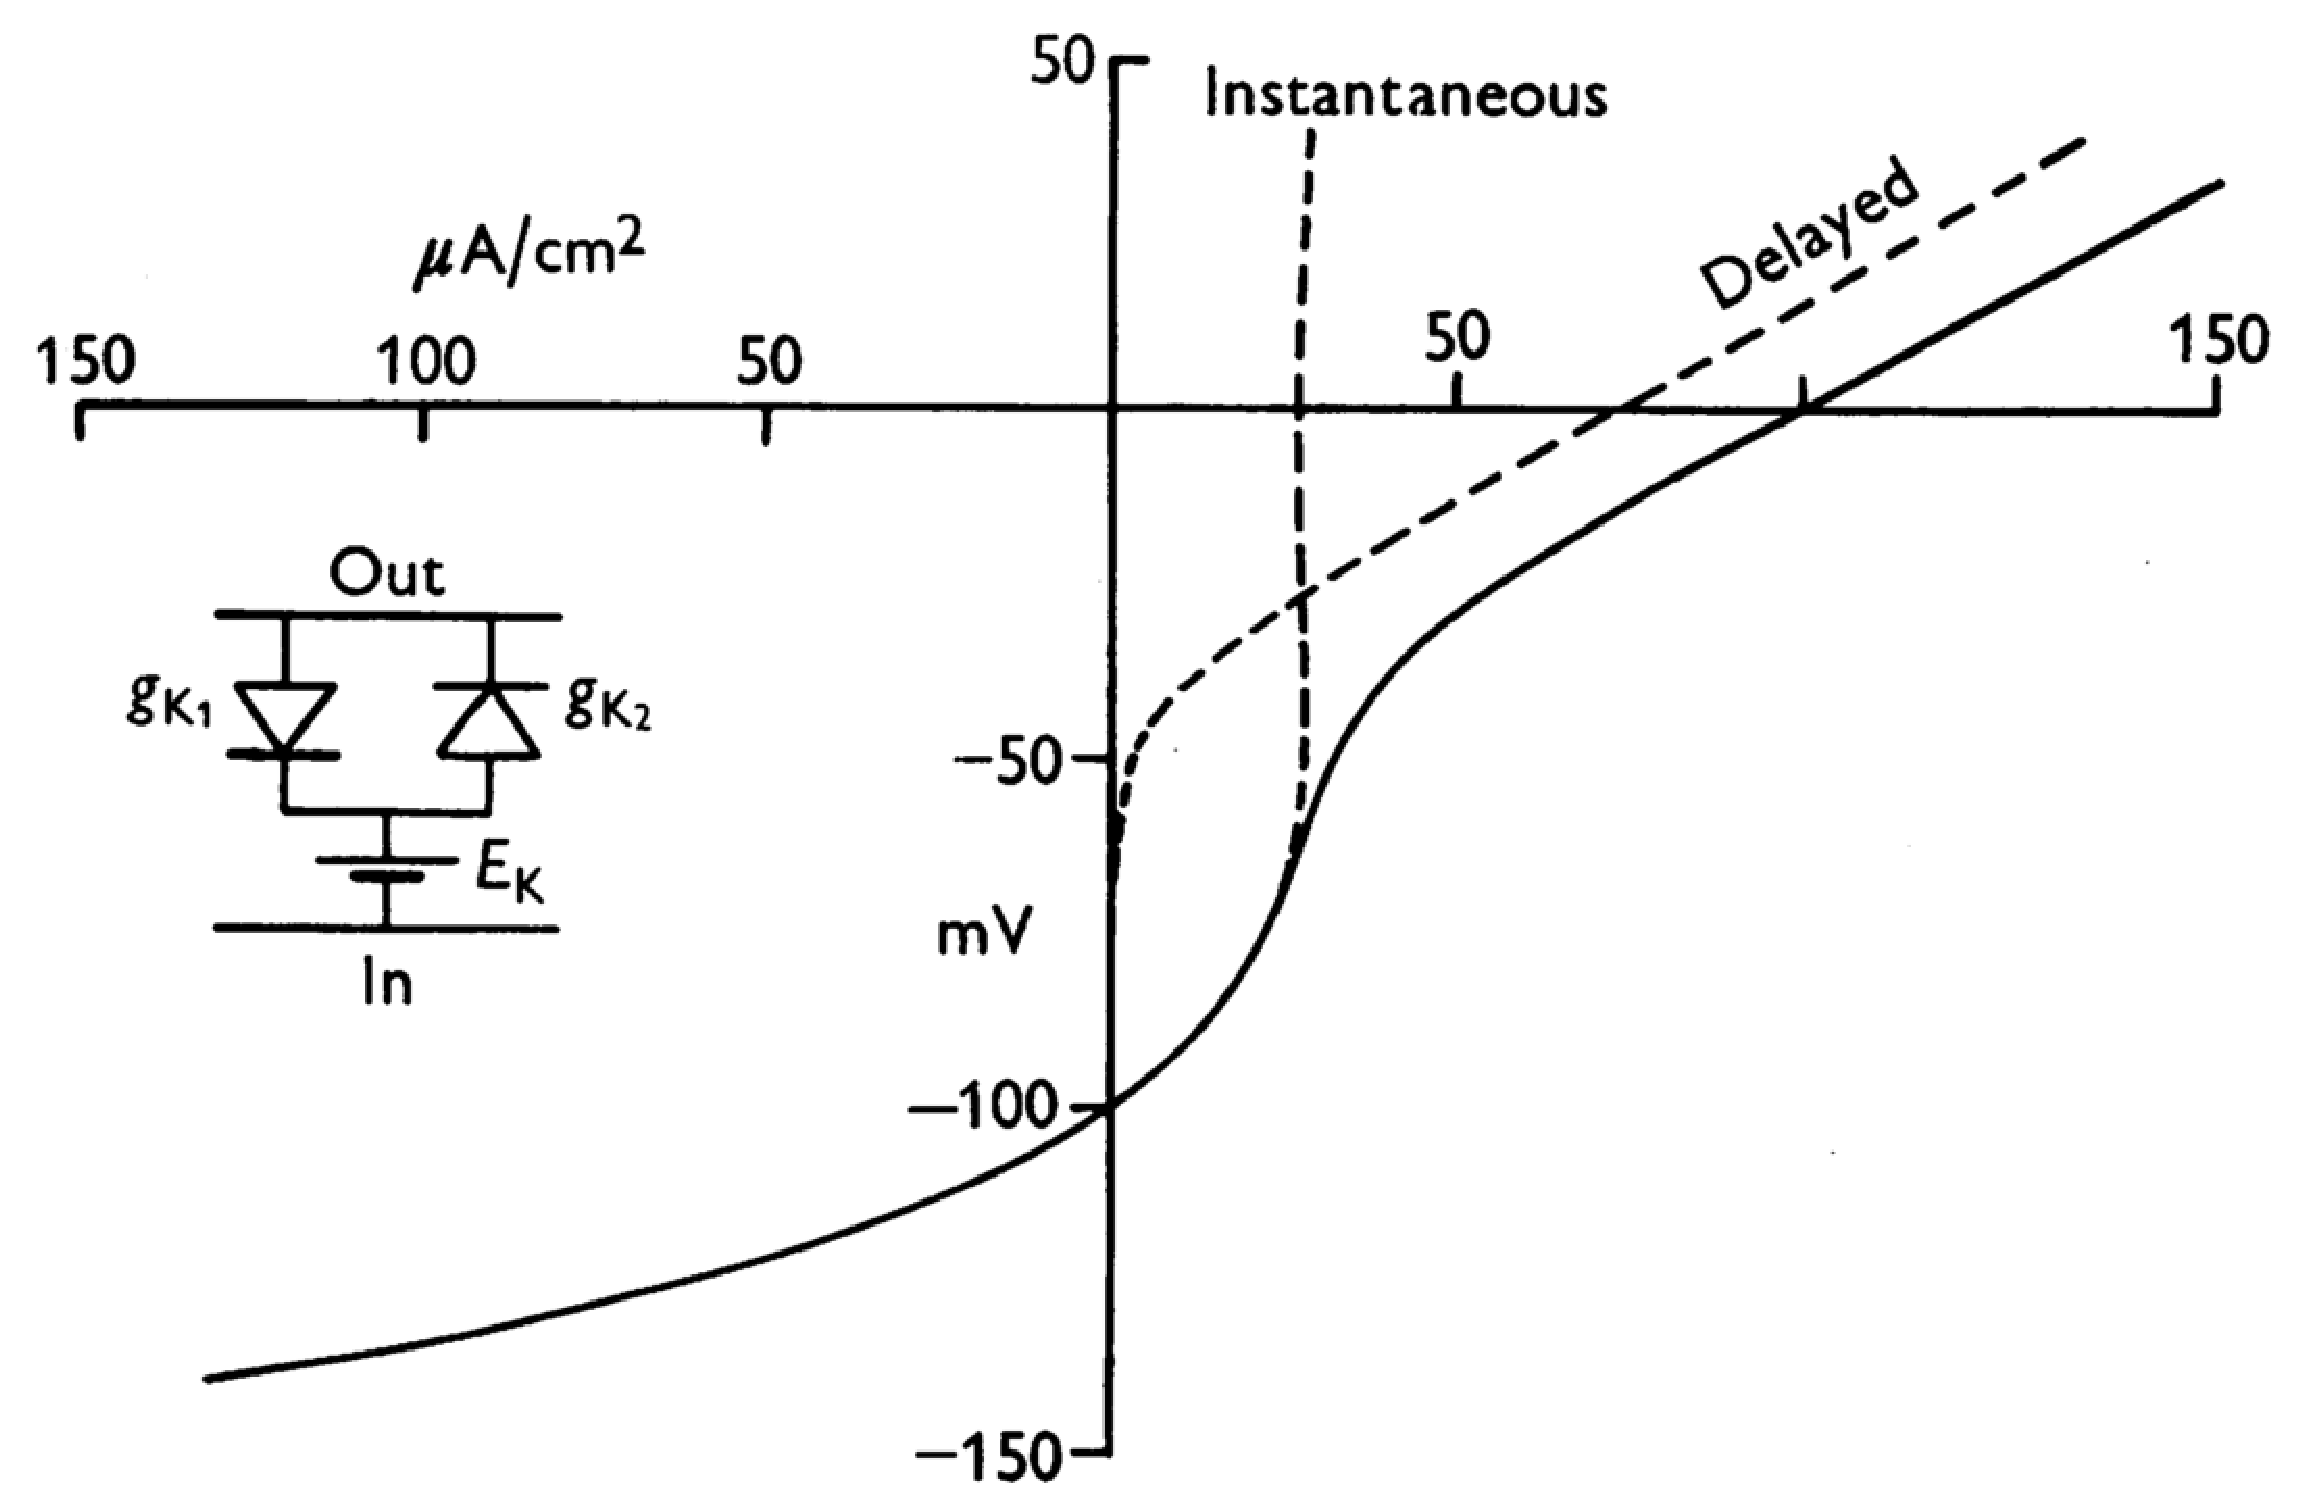
\includegraphics[height=4cm,
    angle=0]{./images/Noble_K.eps}}
\caption{(A) $\K$ current in a $\Na$-deficient solution. The reversal potential
is at -92mV. However, the K current change the direction of the current (from
inward when $V_m<-92$mV to outward when $V_m>-92$mV). (B) $I_\k$-V relation}
\label{fig:Noble_K}
\end{figure}

% \begin{figure}[hbt]
%   \centerline{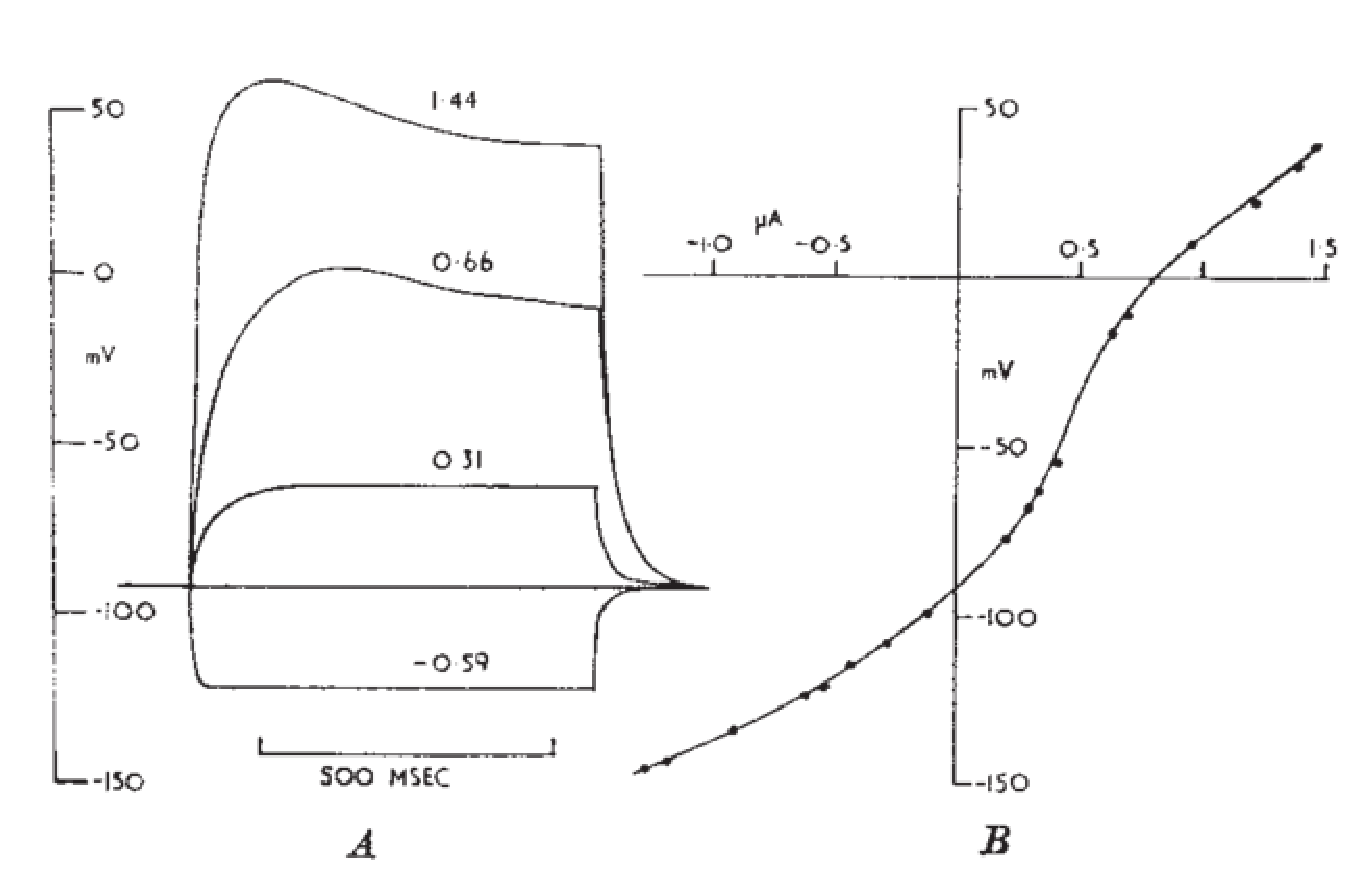
\includegraphics[height=5cm,
%     angle=0]{./images/Hutter1960_Kcurrent.eps}}
% \caption{}
% \label{fig:Hutter1960_Kcurrent}
% \end{figure}
\begin{framed}

The rectification property of an ion channel which means that the
channel can carry the charges inward or outward depending on the membrane
potential. \textcolor{blue}{This is an intrinsic property. Whether the channel
can carry charges inward easier or outward easier, the channel is called
inwardly or outwardly rectifying}. The molecualr mechanism of rectification
varies with ion channel type. 
\end{framed}

The $\K$ current via the delayed rectifier $I_\k$ in axon model is not the same
as that in Purkinje fibre. As the contribution of chlorine ions to the membrane
conductance of cardiac muscle is small, \textcolor{red}{it's assumed that only
sodium and potassium ions involve in regulating membrane potential}.
In a sodium-defficient solutions, Fig.~\ref{fig:Noble_K}, ~\citep{hutter1960}
found out that the membrane conductance is decreased along with the
depolarization. So, the decreases in conductance upon depolarization in the
sodium-free solution is the decrease of $\K$ conductance {\it per se}. However,
as shown in Fig.~\ref{fig:Purkinjie_conduct}, when the potential is suddenly
returned to -92mV, $g_\k$ rises above its resting value, and then slowly fall.
So, it's hypothesized that there must be two K currents: one component with
conductance $g_{K1}$ fall instantly when $V_m$ depolarized and one component
whose conductance $g_{K2}$ increase slowly when $V_m$ depolarized.
Even though the authors pointed out that there can be a delay in $g_{K1}$
following changes in $V_m$, they kept using the assumption of instantaneous
function of $V_m$ change [NOTICE: The experimental data didn't show any
informatin to support the assumption that $I_{K1}$ is an instantaneous function
of $V_m$.]

The equivalent electrical circuit of the Purkinje fibre, given in
Fig.~\ref{fig:circuit_Purkinjie}, has only one difference in the Potassium
conductance with two parallel rectifiers, eq.\ref{eq:541}, which was later
confirmed by \citep{mcallister1966}:
\begin{enumerate}
  \item the $V_m$-dependent inward rectifier $I_{K1}$ (the depolarization
  decreases the permeability of IK1 and then slowly increases during the passage
  of the repolarization). IK1 carries charges inward more easily at negative
  potential.
  
  \item Time-dependent delayed rectifier outward current $I_{K2}$
  (IK2) which slowly activate at depolarized membrane potential, and then
  deactivate with the repolariation. IK2 carries charges outward more easily at
  more positive potential.
\end{enumerate}

The leak current was assumed to conduct anion, so given the name $I_\text{An}$,
rather than $I_\text{leak}$. 
\begin{equation}
I_\text{An}=g_\text{An}(V_m-E_\text{An})
\end{equation}
In Purkinje fibres, the experimental data at that
time shown a very small leak current so it is neglected in the model
$g_\text{An}=0$ (\textcolor{red}{this is indeed not an accurate measurement}).


\begin{figure}[hbt]
  \centerline{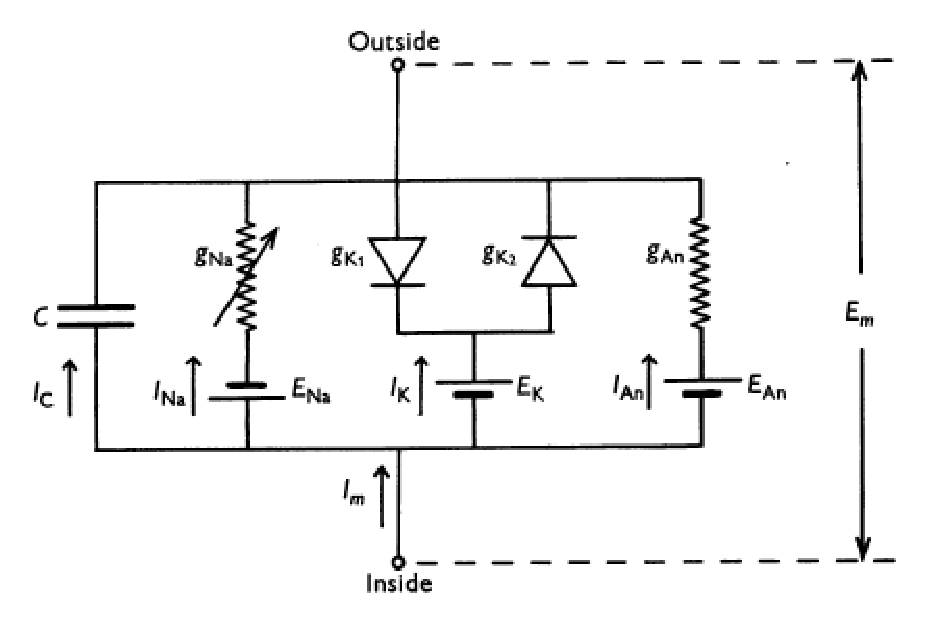
\includegraphics[height=5cm]{./images/circuit_Purkinjie.eps}}
  \caption{Equivalent circuit for Purkinje fibre membrane}
  \label{fig:circuit_Purkinjie}
\end{figure}


% \item In sodium-deficient solutions, it was observed that
%   depolarization in Purkinje fibre doesn't increase as observed in
%   nerve cell, Fig.~\ref{fig:g_K}. Indeed, the membrane conductance
%   first decrease and then slowly rise to the resting conductance; when
%   the voltage clamp is removed, there is an increase in conductance
%   before it restoring back the resting value. As $g_L$ was assumed to
%   be zero, this decrease is mapped to $g_K$ decrease, as shown in
%   Fig. \ref{fig:Purkinjie_conduct}.  Noble hypothesized that there
%   must be an instantaneous voltage-dependent time-independent inward K
%   current that cause the early decrease in conductance, counteracting
%   with the slowly increase voltage-dependent time-dependent outward K
%   current. Then, mathematically, it can be assumed that the $g_K$ is
%   composed of 2 components in parallel,
%   Fig.~\ref{fig:circuit_Purkinjie}:
%   \begin{enumerate}
%   \item one instantaneous (time-independent), voltage-dependent
%     {\it inward} $g_{K1}$.
%   \item one slow (time-dependent), voltage-dependent {\it outward}
%     $g_{K2}$.
%   \end{enumerate}

\begin{framed}
  $g_{K2}$ helps hyperpolarizing the membrane.
  \textcolor{blue}{The plateau in the AP of Purkinje fibre is
    300-400ms while that in axon is only 3ms which is about 100x
    longer}.
  Thus, the kinetics of $g_{K2}$ is 100x slower, to maintain the
  plateau (the depolarizing is slow enough) in the AP shape. For this
  reason, $g_{K2}$ is also called the {\bf delayed rectifier}
  $g_\Kdr$.
\end{framed}

\begin{framed}
  All gating variables ($w=m,n,h$) follow the first-order kinetics
\begin{equation}
  \label{eq:605}
  \frac{dw}{dt} = -\alpha_w(w-w_\infty) -\beta_w
\end{equation}
with $\alpha_w, \beta_w$ are of the form
\begin{equation}
  \label{eq:606}
  \frac{C_1\exp(\frac{V_m-V_0}{C_2})+C_3(V_m-V_0)}{1+C_4\exp(\frac{V_m-V_0}{C_5})}
\end{equation}
\end{framed}

{\bf REMARK}: eq.~\eqref{eq:606} is the special case of
eq.~\eqref{eq:578}. These constants are defined as given in
Fig.~\ref{fig:Noble_rate_constant} (the values denoted by `---' means
the value is not important when $C_1=0$ or $C_4=0$ already).
\begin{figure}[hbt]
  \centerline{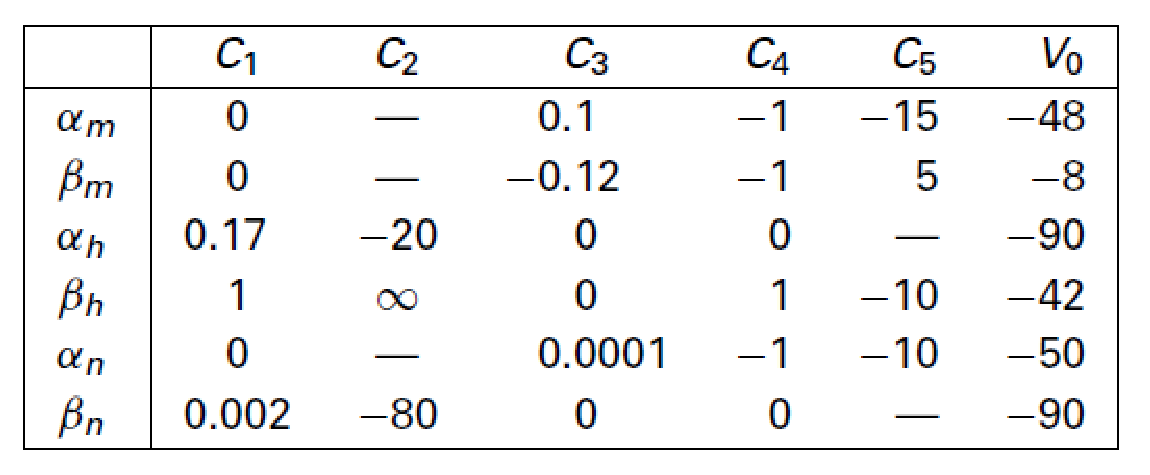
\includegraphics[height=4cm,
    angle=0]{./images/Noble_rate_constant.eps}}
\caption{Rate constants for Noble model}
\label{fig:Noble_rate_constant}
\end{figure}


\subsection{Mathematical model}
\label{sec:mathematical-model-2}

Unit:
\begin{itemize}
\item current : $\mu$A/cm$^2$
\item conductance: mmho/cm$^2$ (or mS/cm$^2$)
\item voltage (inside minus outside): mV
\end{itemize}

\begin{equation}
\Csc\frac{dV_m}{dt} = \sum I_\ion - I_\app
\end{equation}
The model parameters were computed with $\Csc=12\mu$F/cm$^2$ (12 times
larger than that in squid nerve)~\citep{weidmann1952ecp}
(\textcolor{red}{this value is unrealistically large and we will learn
  that the correct one in cardiac cells} is $\Csc\approx 1\mu$F/cm$^2$).
The absolute conductance was adjusted to give the conductance at resting
potential ($V_\rest=-90$mV) is 1mmho/cm$^2$.

\begin{enumerate}
  
\item {\bf Model $I_K$}: 2 components inward rectifier K1 and outward
rectifier K2.
  \label{sec:potassium-current-1}

  \begin{eqnarray}
    \label{eq:541}
    I_{\ce{K}} = (g_{K_1}+g_{K_2}) (V_m-E_{\ce{K}})
  \end{eqnarray}
  with $E_\k=-100$mV. The purely empirical equation for the inward Kv
  current $g_{K_1}$ is modeled as a sum of two exponential functions (i.e. two
  parralel rectifiers)
  \begin{equation}
    \label{eq:355}
    g_{K_1} = 1.2 \exp\left[-\frac{V_m+90}{50}\right] + 0.015 \exp\left[\frac{V_m+90}{60} \right]
  \end{equation}
%   or
%   \begin{equation}
%     \label{eq:356}
%     g_{K_1} = 1.2 \exp\left[-\frac{v}{50}\right] + 0.015 \exp\left[\frac{v}{60} \right]
%   \end{equation}
%   with $v=V_m-E_{K}$.

  The conductance $g_{K_2}$ is described using that of Hodgkin-Huxley given the
  maximum conductance $\overline{g_{K_2}}=1.2$ (mmho/cm$^2$), a much smaller
  value than the conductance of potassium channel in nerve cell (36
  mmho/cm$^2$).  This is to guarantee that the increase in $g_{K_2}$ during the
  depolarization should not offset the decrease in $g_{K_1}$, i.e. giving a
  decrease in the total $\K$ conductance.   In addition, to take into account
  the very slow onset (i.e. a delay) of this current, the rate constants are
  made smaller by dividing them by 100, e.g. $\alpha_n, \beta_n$ are divided by
  a factor of $p=100$.
  \begin{equation}
    \label{eq:357}
    \begin{split}
      g_{K_2} &= 1.2\times n^4 \\
      \frac{dn}{dt} &= \alpha_n(1-n) - \beta n \\
      \alpha_n &= \frac{-0.01(V_m+50)}{p\times (\exp\left[
      -\frac{V_m+50}{10}\right] - 1)} \\
      \beta_n &= \frac{0.2\exp \left[ - \frac{V_m+90}{80}\right]}{p}
    \end{split}
  \end{equation}
 
\item {\bf Model $I_{Na}$}: It's assumed there's a small component of $\Na$
current ($g_i = 0.14$mmho/cm$^2$) independent from $V_m$ to account for the
plateau range in AP
  \label{sec:sodium-current}
  \begin{equation}
    \label{eq:607}
    I_{\ce{Na}} = (g_{Na}+g_i)(V_m-E_\na)   
  \end{equation}
with $E_\na=40$mV, and
  \begin{equation}
    \label{eq:57}
    \begin{split}
      g_{\ce{Na}} &= m^3h\overline{g_{\ce{Na}}}\\
      \frac{dm}{dt} &= \alpha_m(1-m) - \beta_m m \\
      \frac{dh}{dt} &= \alpha_h(1-h) - \beta_h h
    \end{split}
  \end{equation}
with $\overline{g_\na}=400$mmho/cm$^2$.

  Inactivation gating variables $\alpha_h, \beta_h$ was assumed to be the same
  as those of K channels in squid axon, i.e. the curves have the same shape,
  except that the relation between $V_m$ and the steady-state value need to be
  adjusted to give $V_m(h_\infty=0.5)=-71$mV) \citep{weidmann1955cmp}. The
  constants in the formula were adjusted to give the desired relationship  
  \begin{equation}
    \label{eq:358}
    \begin{split}
      \alpha_h &= 0.17 \exp (-\frac{V_m+90}{20})  \\
      \beta_h &= \frac{1}{\exp(-\frac{V_m+42}{10}) + 1}
    \end{split}
  \end{equation}
  
  Activation variables is very steep. Using voltage-clamp technique, when $\Na$
  increases, it was impossible to retain the control of $V_m$, thus data for the
  activation of $\Na$ current was unavailable. Giving the shape of AP and
  equations for $h$ (above) and $I_\k$, what equations should be used for
  $\alpha_m, \beta_m$ to describe $m$??? The approach was described in
  ``Methods" section of the paper in which $m$ was plotted against $V_m$ (given
  that other currents was known using the formula given above). The empirically
  chosen formula was
  \begin{equation}
    \label{eq:359}
    \begin{split}
      \alpha_m &= \frac{-0.1(V_m+48)}{\exp(-\frac{V_m+48}{15})-1} \\
      \beta_m &=  \frac{0.2(V_m+8)}{\exp(\frac{V_m+8}{5})-1}
    \end{split}
  \end{equation}

%   The small component $g_i = 0.14$ mmho/cm$^2$ is independent of $V_m$
%   and $t$. $\overline{g}_{\ce{Na}}=400$ mmho/cm$^2$ and $E_{\ce{Na}}=40$mV.


\end{enumerate}


\subsection{Numerical analysis}
\label{sec:numerical-analysis-4}

The simulated was performed on ``Mercurry'' digital computer at London
University, with Runge-Kutta numerical method. The time step $\Delta
t=0.1$ms. Data is written out at every 10 time steps. What to print out?
$t, V_m, m,h,n,g_\na, g_\k$ and Fluxes ($\Na$ efflux, $\Na$ influx, $\K$
efflux, $\K$ influx, net $\Na$ gain, net $\K$ loss).

NOTE: The system become unstable when we use $\Delta t > 2.8 T_\min$,
with $T_\min$ is the smallest time constant in the system
(e.g. $\tau_m, \tau_n,...$ with m, n... are gating variables). 

\textcolor{blue}{Noble model has 4 variables} ($V_m, n, m, h$).  The
constants given in the above equations are determined using
$h_\infty=0.5, m_\infty=0.5$. A guess was given for
$n_\infty=0.72$. This causes the first cycle to be error, and we have
to consider the value from the second cycle.

An initial potential $V_m$ can be chosen at about the middle of the pace-maker
potential, when $dV_m/dt$ is very small. Then, the initial values for $m, n$,
and $h$ are assigned to $m_\infty, n_\infty$, and $h_\infty$, without any
appreciable error. Try with $V(0)=-71mV, -90mV$.


\subsection{Data Analysis}
\label{sec:analysis-5}

Experimental data: \citep{weidmann1955cmp} ($\Na$ current).

{\bf XPPAUT code} (Chap.\ref{chap:XPPAUT}): \hyperref[Noble_model]{code}


\begin{figure}[hbt]
  \centerline{\includegraphics[height=5cm, angle=-90]{./images/Noble_model_V_t.eps},\includegraphics[height=5cm, angle=-90]{./images/Noble_model_gK_gNa.eps}}
  \caption{(A)Membrane potential during the time course, (B) The time
    course of the conductances of sodium and potassium channels}
  \label{fig:Noble}
\end{figure}

% \begin{figure}[hbt]
%   \centerline{\includegraphics[height=5cm, angle=-90]{./images/Noble_model_gK_gNa.eps}}
%   \caption{The time course of the conductances of sodium and potassium
%     channels}
%   \label{fig:Noble_N_Ka}
% \end{figure}

\begin{figure}[hbt]
  \centerline{\includegraphics[height=5cm, angle=-90]{./images/Noble_model_m_h.eps}}
  \caption{$m$ and $h$, $m$ rises much faster than $h$}
  \label{fig:Noble_m_h}
\end{figure}


\begin{enumerate}
\item As a pace-maker, the AP of the Purkinje fibre oscillate.  The AP
  requires no externally applied current, all the current being
  supplied by the fibre itself, i.e. there are AP even the initial
  potential is lower than the resting potential.
\item Each cycle is around 500ms. The analyze should be taken from the
  second cycle as there is a noncritical error in the first cycle due
  to the guess of $n(0)$.
\item The conductance change in sodium is instantaneous, while that in
  potassium has a delay and slow. However, right after the quick
  increase (``undershoot'') in conductance, the $g_{\ce{Na}}$ falls back
  to a lower value, yet the inactivation is not complete. In other
  words, $g_{\ce{Na}}$ stay at a fairly constant plateau of about 8
  times its resting value..
\item $g_{\ce{K}}$, by contrast, stay below its resting value during the
  plateau, and it increases slowly~\citep{noble1960cap}.
\end{enumerate}


% To account for the long-lasting action potential, many modification to
% the Hodgkin-Huxley equations have been done.  The maximum rate
% ($100mV/sec$) is much slower than that measure experimentally
% ($300mV/sec$).


\subsection{Summary}
\label{sec:summary-4}

The equivalent electrical circuit of the Purkinje fibre, given in
Fig.~\ref{fig:circuit_Purkinjie}, has only one difference in the
Potassium conductance with two parallel rectifiers.  Even though the
shape of the AP is correct, some underlying physiological properties
was not correct. The main reason is that voltage-clamp data for
cardiac membrane was not available until 1964.
\begin{itemize}
\item Even though Noble was correct when consider \ce{Na+} as the main
  charge carriers during the upstroke of the AP in Purkinje fiber, he
  was wrong when consider potassium conductance $g_{K2}$ as the
  carrier in charge of the plateau in AP. In deed, it is the slow
  outward calcium current. This is resolved in a different model,
  McAllister-Noble-Tsien model (1962) (read
  Sect.~\ref{sec:macall-noble-tsien}).

\item The capacitance $\Csc=12 \mu$F/cm$^2$ is unrealistically
  large. This value was used by Noble as it gives the correct time
  scale for the length of the AP. The correct one should be
  $\Csc=1\mu$F/cm$^2$
\end{itemize}

The two-variable FitzHugh-Nagumo model can not produce the sharp spike
in the early AP.  The Noble model also has the same variables with
Hodgkin-Huxley model.  Nowadays it is clear that the current is also
produced by electrogenic pumps (e.g. \ce{Na+}/\ce{K+}-pump), they had
not been taken into account in this model. Read
Chap.~\ref{chap:models-pumps} for more detail on pump and exchanger
models. Thus, this model is far from
complete. % In other words, all changes in conductances that were measured
% in sodium deficient solution were assumed to be currents carried out
% by potassium ions.  


\section{McAllister-Noble-Tsien model (1975)}
\label{sec:macall-noble-tsien}


\subsection{Hipothesis analysis}
\label{sec:hipothesis-analysis}

In 1962, Noble proposed a model for Purkinje fibre
(Sect.~\ref{sec:noble-model}), based on Hodgkin-Huxley model for nerve cell,
with only 3 ionic currents (4 variables). With new experimental results,
Trautwein (1973) and Noble (1974) believed that the number of ionic components,
each serves at least a functionality  distinct for electrical activity is much
greater than in nerve cells.  Thus, MNT model suggested 9 different ionic
currents, giving 9 gating variables~\citep{mcallister1975rea}.

\textcolor{green}{First assumption is the uniform cross-sectional
  distribution of both capacitance and ionic currents in the cylindrical surface
  and T-tubule}.
Otherwise, one area of membrane will depolarize faster and thus non-uniformities
will then appear. \textcolor{green}{Then, it's assumed membrane of isopotential}
(i.e. uniform action potential) $dV_m/dt=-(I_\ion)/\Csc$. The experimental data
used for this model were measured from the cylindrical surface area,
$\Csc=10\mu$F/cm$^2$ (which is incorrect -
\ref{{sec:specific-membrane-capacitance}}).

% Under normal physiological condition, the sodium current is too high for the
% voltage-clamp to work. So, to obtain the dynamic of Na channels, its
% activation was slowed by the cool down of temperature (4-5$^o$C). Then, it's
% observed that Na channels in Purkinje fibre has can be fitted by
% Hodgkin-Huxley formula, yet with a different voltage dependent.
As mentioned in Sect.\ref{sec:noble-model}, accurate measurement of the
magnitude $\bar{g_\na}$ of $I_\na$ was not possible as the kinetics is extremely
fast. Thus, similar to the approach of Noble model (1962), Na current was
assumed to be similar to that in squid axon (biphasic behavior). The
time-dependent Na current is modeled by Hodgkin-Huxley formula with two gating
variables, yet with a different voltage dependent, eq.~\eqref{eq:608}. The
background Na conductance is now called $g_{Na,b}$, rather than $g_i$ as in
Noble model, eq.~\eqref{eq:615}.

In addition to the transient inward Na current, there is another inward current,
with slower kinetics, called secondary-inward current $I_{si}$ which is carried
partially by calcium current~\citep{johnson1971hec, reuter1973dcc}\footnote{some
people call it slow-inward current; it definitely slower than sodium current;
but faster than Ix1 and Ix2. So, it's better to use the work 'secondary' than
'slow'}. It's aka 'negative dynamic current' (due to its inward current
property), while the current $I_\text{qr}$ is called 'positive dynamics current'
\citep{trautwein1973mcc}.  This current is activated by a step depolarization
from -80mV passing the threshold -50 mV which is far beyond the threshold of Na
current, and reaches the peak in 5-10ms. To reconstruct the current, they used
the linear relation
    \begin{eqnarray*}
      i_{si} = \overline{g}_{si}(V_m-E_{si})
    \end{eqnarray*}
with $\overline{g}_{si}=0.8$mmhos/cm$^2$, and reversal potential $E_{si}=+70$mV.     
The activation stage was not clear, so the authors hypothesized of
$d$ raised to the first power, with $d$ is identical in form to $m$ of $\Na$
channel, but slower ($\tau_d=12$msec at 0mV and $d_\infty=0.5$ at -40mV). 
\citep{vitek1971} used $d_\infty=0.5$ at -20mV; so they suggested that there're
some variations between fiber position in the half-maximal curve of
$d_\infty(V_m)$. In addition, experiments shown that the inactivation is not
completed, i.e. 
about one fifth to one half of the current still active even at a prolonged
depolarization. To model this residual current, a residual time-independent
component of the secondary inward current with maximum conductance
$\overline{g'_{si}}$ is required with a Voltage-dependent time-independent
gating variable $d'$ in eq.~\eqref{eq:609}.

Unlike Noble model's assumption, the chlorine was taken into account with two
different currents. The small chlorine currents $I_{\cl,b}$ was found contribute
to shortening the plateau of the AP, and accelerating the rate of pacemaker
depolarization.  In addition, there is also a larger chlorine current, denoted
as $I_{qr}$, eq.\eqref{eq:611}, which functions as a transient outward current
to contribute to the transient early repolarization of AP to the beginning of
the plateau.

In Noble (1962) model, two different $\K$ currents were assumed in the model:
$V_m$-dependent inward rectifier $I_{K1}$, and time-dependent delayed rectifier
outward current $I_{K2}$ ($I_\k$). $I_{K2}$ has the reversal potential at the
very negative value (about -90 mV) and full active at -60mV
~\citep{noble1968krp}. Later on, at the plateau range of membrane potential,
another time-dependent $\K$ current $I_x$ was also found \citep{noble1969omc}.
However, this current is less selective to potassium than the current at
negative potential, and thus has a small contribution. When membrane voltage
depolarize over -20mV, the current recorded become more complicated and more
components appear. As a result, it was thus hypothesized that there are two
components of $I_x$:  fast component $I_{x1}$ (turn on at -50mV) and slow
component $I_{x2}$ (turn on at -40 mV)\footnote{both fully activated at the
steady-state at +20mV}~\citep{noble1969omc}. In essence, there are three
time-dependent $\K$ outward current in the model: $I_{K2}, I_{x1}, I_{x2}$, with
the current-voltage characteristics given in Fig.~\ref{fig:MNT_out_current}.

\begin{enumerate}
  \item  The first component, still denoted as $I_{K2}$, is a highly non-linear
  process. It marked an inward-going rectification with a negative slope
  conductance appearing at voltage 20-30mV more positive than $E_\k$. This
  negative slope conductance persists at strong depolarization so that the
  current tends toward zero at about 0mV. The formula inward delay-rectifier
  $I_{K2}$ was derived from the equation developed by
  eq.15.1 in ~\citep{adrian1969rms}, eq.~\eqref{eq:699}.

\begin{equation}
  \label{eq:698}
  g_{K2} \varpropto s^\gamma
\end{equation}
with $\gamma=1$. Here, $s$ is used rather than the notation $n$ in
nerve cell K current because the kinetics of $s$ are generally
two-order slower than $n$ kinetics\footnote{$s$ is the fraction of total
$g_{K_2}$ which is activated. }.
$s_\infty$ is zero at $V_m=-90$mV and reaches 1 at $V_m=-60$mV.

\item $I_{x1}$ is also based on Adrian model for inward delay-rectifier, yet
with parameter values preventing the current from declining to zero at large
depolarization~\citep{adrian1969rms}, eq.\ref{eq:612}.
\begin{figure}[hbt]
  \centerline{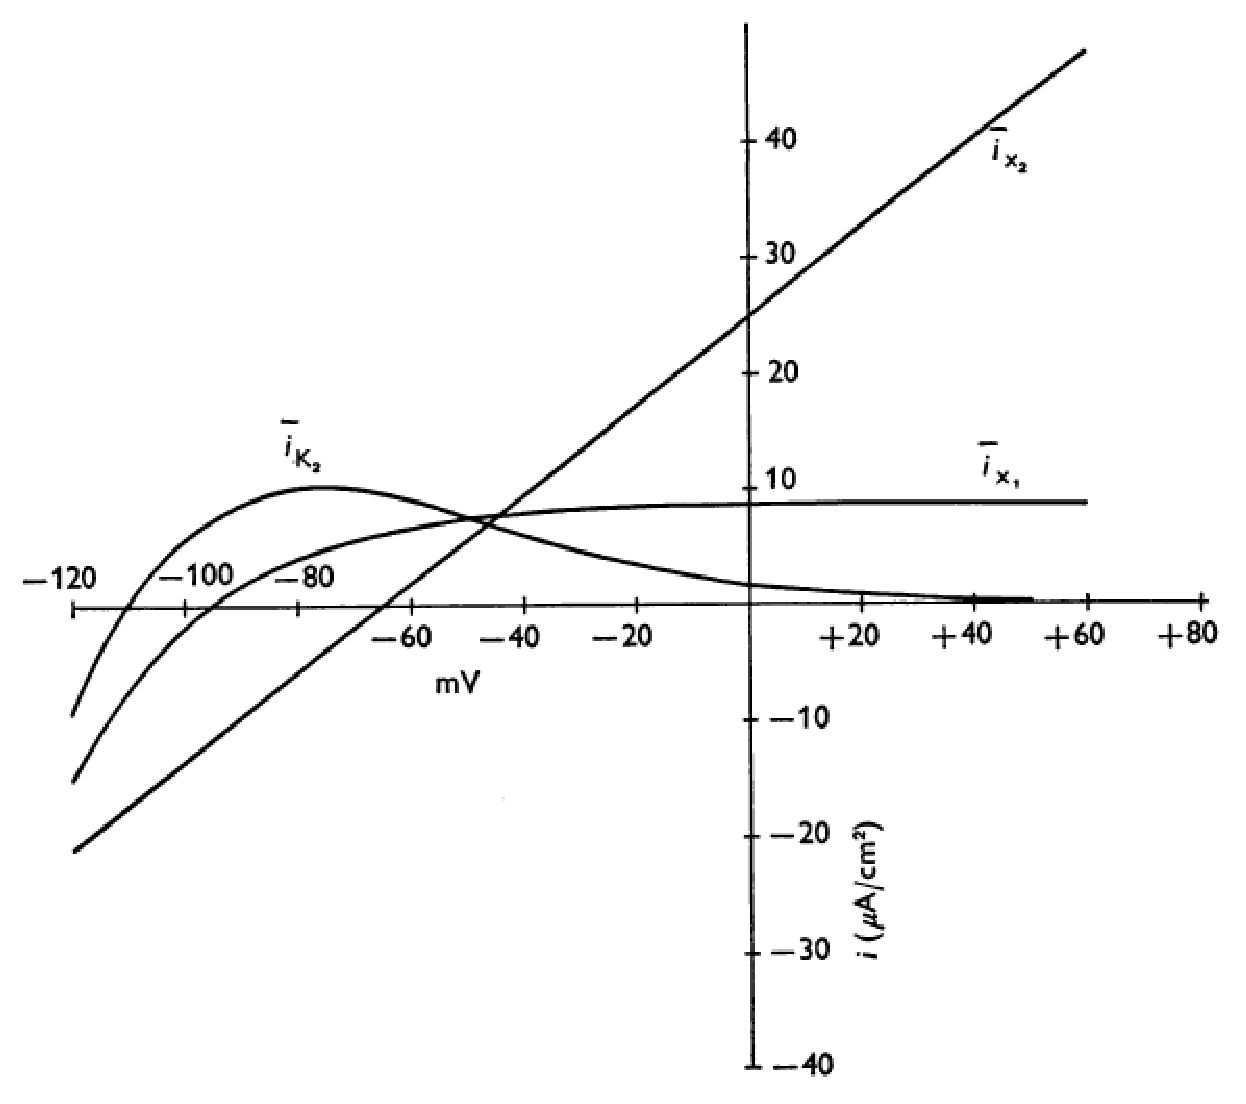
\includegraphics[height=5cm,
    angle=0]{./images/MNT_current.eps}}
  \caption{I-V characteristic of outward current components: one for
    each component when its channels are fully open (gating variable equal to
    1)}
  \label{fig:MNT_out_current}
\end{figure}

\end{enumerate}

\begin{framed}
Inward rectification is an important property of cardiac, skeletal
muscles and neurons. Rectification depends on $[K]_o$ and occurs
around $E_K$ (reversal potential of K channels). It means that K entry
dominates K outward around $E_K$. This K entry maintains a long
plateau in AP, contributing a major role in cardiac pacemaker
activity, and regulating firing frequency~\citep{rudy1988duk}.

Later on, $I_{x1}$ is known as the fast component $I_\Kr$ carries an
inward-going rectification at instantaneous change in potential, and $I_{x2}$ is
the slow component $I_\Ks$ \citep{sanguinetti1990tcc}. They don't have
voltage-dependent bursting behavior. $I_\Ks$ has a linear I-V relationship, and
$I_\Kr$ is preferentially blocked by class III antiarrhythmic compounds.
\end{framed}

$I_{K1}$ the depolarizing-activated inward current (\textcolor{red}{this
should be a hyperpolarizing-activated inward current - corrected in
DiFrancesco-Noble model (1985)}) is now called the outward background $\K$
current eq.~\eqref{eq:614}. Again, the formula is based on Adrian's
rectification model with the additin of a 'constant field' component
($\overline{i_{K1}}/2.8$) at large depolarization.

The background current\footnote{the term ``background'' is used rather than
``leak'' used in HH model as in cardiac electrophysiology, ``leak current''
refer to the current flow in damaged region} is modeled as three components:
outward $I_{K1}$, inward $I_{Na,b}$ and a chlorine background
$I_{\cl,b}$\footnote{The chlorine background current was neglected in
  Noble model (1962).}.
$I_{K1}$ was recorded for the current below the threshold for $I_{x1}$
in sodium-free condition (when $I_{K2}$ is almost zero) and has
inward-going rectification (as assumed by Noble model (1962, though
here it is considered as an outward current), eq.~\eqref{eq:614}. The
reason of adding $I_{Na,b}$, eq.~\eqref{eq:615}, is that the resting
membrane potential (from -90 mV to -80 mV) is higher then the reversal
potential of $K1$ channel (from -115 mV to -100 mV) which is normally
assumed the value of resting potential. Even though the ionic basis of
this inward current is not clear, it was assumed to be sodium influx.
The background chlorine current was chosen to give the AP of duration
400 ms, eq.~\eqref{eq:616}.

\subsection{Mathematical model}
\label{sec:mathematical-model-5}


\begin{itemize}
\item (2) three inward
  currents\footnote{in squid nerve HH model, there is only one sodium
    inward current},
  each with biphasic behavior, i.e. activation and then deactivation
  during
  depolarization\footnote{thus, each one requires 2 gating variables}:
  \begin{enumerate}
  \item sodium currents that resemble HH model
    \begin{equation}
      \label{eq:608}
      I_{Na} = \overline{g_{Na}}m^3h(V_m-E_{Na})
    \end{equation}
    with $E_{Na}=+40$ mV, $\overline{g_{Na}}=150$ mmho/cm$^2$ (to give the
    maximum $i_\na \sim 4\muA/$cm$^2$).  The gating variables (unit:
    sec$^{-1}$). The equations fit best to the data of \citep{noble1962mhh} when
    $[\Ca]_o=2.6$mM, instead of standard 1.8mM. 
\begin{eqnarray}
  \alpha_h &&= 0.0085 \times 10^3 \exp [-(V_m+71)/5.43] \\
  \beta_h &&= 2.5\times 10^3/(\exp[-\frac{V_m + 10}{12.2}] + 1) \\
  \alpha_m &&= \frac{10^3(V_m+47)}{1-\exp[-0.1(V_m+47)]} \\
  \beta_m &&= 40\times 10^3 \exp\left[ -(V_m+72)/17.86 \right] \\
\end{eqnarray}
NOTE: \citep{adrian1970} used the following for striated muscle     
\begin{eqnarray}
  \alpha_h &&= 1.13\times 10^{-4} \exp [-(V_m+10)/5.43] \\
  \beta_h &&= 2.5\times 10^3/(\exp[-\frac{V_m + 10}{12.2}] + 1) \\
  \alpha_m &&= \frac{10^3(V_m+47)}{1-\exp[-0.1(V_m+47)]} \\
  \beta_m &&= 9.86\times 10^3 \exp\left[ -(V_m+72)/17.86 \right] \\
\end{eqnarray}

  \item ``slow-inward'' current $I_{si}$ (which is called calcium current in
  later models): has linear I-V relation and extroplated reversal potential is
  in the range +40mV to +60mV. So, they chose $E_{si,\rev}=+70$mV.
%   This linear relation was modeled as
%     \begin{eqnarray*}
%       i_{si} = \overline{g}_{si}(V_m-E_{si})
%     \end{eqnarray*}
%     Lower than this voltage range, the activation/inactivation stage
%     was not clear, so the authors hypothesized of two gating variables
%     $d,f$. Due to its uncompleted inactivation, $I_{si}$ was modeled
%     as
    \begin{equation}
      \label{eq:609}
      I_{si} = (\overline{g_{si}}.d.f + \overline{g'_{si}}.d') (V_m-E_{si})
    \end{equation}
    $\overline{g_{si}}=0.8$ mmho/cm$^2$,
    $\overline{g'_{si}}=0.04$ mmho/cm$^2$. The parameter values were
    chosen so that the residual component of $I_{si}$ is roughly 6$\mu$A/cm$^2$
    at -40 mV\footnote{it can be interpreted that a certain fraction of Ca
      channels (with a different maximum conductance $\bar{g'}_{si}$) lack the
      property of inactivation}.
    
    The gating $d,f$ are time-dependent activation and inactivation variables,
    respectively (unit: sec$^{-1}$).
    \begin{eqnarray}
      \alpha_d &&= \frac{0.002 \times
      10^3 (V_m+40)}{(1-\exp[-\frac{V_m+40}{10}])}
      \\
  \beta_d &&= 0.02\times 10^3 \exp [-\frac{V_m + 40}{11.26}] \\
  \alpha_f &&= 0.000987\times 10^3 \exp [-\frac{V_m + 60}{25}] \\
  \beta_f &&= \frac{0.02 \times 10^3}{(\exp [- \frac{V_m + 26}{10.2}] + 1)} \\
    \end{eqnarray}
    
    $d'$ is time-independent and is nearly coincides with $d_\infty$; so it can
    be assumed that a fraction of channel simply lack the property of
    inactivation; while the activation mechanism nearly coincides with
    $d_\infty=\frac{\alpha_d}{\alpha_d+\beta_d}$.
    \begin{equation}
      \label{eq:610}
      d' = \frac{1}{1+\exp(-0.15(V_m+40))}
    \end{equation}
  \end{enumerate}

NOTE: \citep{adrian1970} used this formula
    \begin{eqnarray*}
      \alpha_d &&= \frac{0.002 \times
      10^3 (V_m+40)}{(1-\exp[-\frac{V_m+40}{10}])}
      \\
  \beta_d &&= 0.02\times 10^3 \exp [-\frac{V_m + 40}{11.26}] \\
  \alpha_f &&= 0.00253 \times 10^3 \exp [-\frac{V_m + 26}{25}] \\
  \beta_f &&= \frac{0.02 \times 10^3}{(\exp [- \frac{V_m + 26}{11.49}] + 1)} \\
    \end{eqnarray*}

\item (1) chlorine current $I_{qr}$
  \footnote{in nerve cell, chlorine current is the leak current with
    no dynamic behavior, yet in Purkinje fibre, it also shows a dynamic
    behavior} that show a dynamic biphasic behavior at high depolarization
  \begin{equation}
    \label{eq:611}
    I_{qr} = \overline{g_{qr}} .q.r.(V_m-E_{\cl})
  \end{equation}
  $\overline{g_{qr}}=2.5$ mmho/cm$^2$, $E_{\cl}=-70$ mV, and $q$ is
  activating variable, $r$ is inactivating variable. Little data was
  available for the estimation of activation process, thus they assume
  it is proportional to $q$ to the first-order (unit: sec$^{-1}$).
\begin{eqnarray}
  \alpha_q &&= \frac{0.008\times 10^3 V_m}{(1-\exp[-0.1 V_m])} \\
  \beta_q &&= 0.08 \times 10^3 \exp[- \frac{V_m}{11.26}] \\
  \alpha_r &&= 2.08\times 10^{-2} \exp[-0.04(V_m + 26)] \\
  \beta_r &&= \frac{0.02\times 10^3}{(\exp[ -\frac{V_m + 26}{11.49}] +1)} \\
\end{eqnarray}
NOTE: \citep{fozzard1973} suggested a different set of values for the 'r'
variables
\begin{eqnarray*}
  \alpha_r &&= 1.93\times 10^{-1} \exp[-(V_m + 30)/17] \\
  \beta_r &&= \frac{0.033\times 10^3}{(\exp[ -\frac{V_m + 30}{8}] +1)} \\
\end{eqnarray*} 

\item (3) three outward potassium currents: $I_{K2}, I_{x1}$, $I_{x2}$. As shown
  in Fig.~\ref{fig:MNT_out_current}, $I_{x2}$ displays a linear
  relation for the fully activated current; while $I_{K2}$ display an
  inward-going rectification. 
  The three components obey a simple first-order kinetics, i.e. each has one
gating variable in the formula for each current (IK2, Ix1, Ix2), i.e. s, x1
and x2 correspondingly (unit: sec$^{-1}$).
    \begin{equation}
      \label{eq:699}
      \begin{split}
        I_{K2} &= \overline{I_{K2}}.s \\
        \overline{I_{K2}} &= \frac{ 2.8(\exp[0.04(V_m +110)]-1)}{(\exp[0.08(V_m + 60)]
          +\exp [0.04(V_m + 60)])} \\
      \end{split}
    \end{equation}
with $E_{\k2}=-110$mV (at $[\K]_o=2.7$mM). 
\begin{equation}
  \label{eq:613}
  \begin{split}
    \alpha_s &= \frac{0.001 \times 10^3 (V_m + 52)}{1-\exp[-\frac{(V_m +
    52)}{5}]}
    \\
    \beta_s &= 5\times 10^{-2} \exp[-\frac{V_m + 52}{14.93}]\\
  \end{split}
\end{equation}

Ix2 found to obey a linear-relationship to $V_m$, with a reversal potential
$E_\rev=-65$mV \citep{noble1969omc}. 
\begin{equation}
  \label{eq:612}
  \begin{split}
    I_{x1} &= \frac{1.2(\exp [0.04(V_m + 95)]-1 )}{(\exp [0.04(V_m +
      45)])} .x1 \\
    I_{x2} &= (25+0.385V_m).x2
  \end{split}
\end{equation}
with $E_{x1}=-84$mV (at $[\K]_o$=4mM) (or -95mV when adjusted to 2.7mM);
$E_{x2}=-65$mV. The gating variables begin to turn on at about -50 mV (Ix1), and
-40mV (Ix2) and fully activated at about +20mV. 
\begin{eqnarray}
    \alpha_{x1} &&= \frac{5\times
    10^{-1}\exp\frac{V_m+50}{12.1}}{1+\exp[\frac{V_m+50}{17.5}]} \\
    \beta_{x1} &&= \frac{0.0013\times 10^3
      \exp[-\frac{V_m+20}{16.67}]}{1+\exp[-\frac{V_m+20}{25}]} \\
    \alpha_{x2} &&= \frac{1.27\times 10^{-1}}{
      1+\exp[-\frac{V_m+19}{5}]} \\
    \beta_{x2} &&=  \frac{3\times 10^{-1}
      \exp[-\frac{V_m+20}{16.67}]}{1+\exp[-\frac{V_m+20}{25}]}
\end{eqnarray}

\item (3) the background current has three components:
  \begin{itemize}
  \item inward $I_{K1}$
    is based on Andrian~\citep{adrian1969rms} with the addition of a
    constant field at large depolarization.
    \begin{equation}
      \label{eq:614}
      I_{K1} = (\overline{I_{K1}}/2.8) + \frac{0.2(V_m + 30)}{(1- \exp[ - 0.04(V_m + 30)]}
    \end{equation}
    with $\overline{I_{K1}}=\overline{I_{K2}}$.

  \item inward Na current $I_{Na,b}$:
    \begin{equation}
      \label{eq:615}
      I_{Na,b} = \overline{g_{Na,b}}(V_m-E_{Na})
    \end{equation}
    with $\overline{g_{Na,b}}=0.105$ mmho/cm$^2$, $E_{Na}=40$mV.
  \item chlorine current $I_{\cl,b}$:
    \begin{equation}
      \label{eq:616}
      I_{\cl,b} = \overline{g_{\cl,b}} (V_m-E_{\cl})
    \end{equation}
with $\overline{g_{\cl,l}}=0.01$ mmho/cm$^2$ (chosen arbitrarily to give the
AP of duration 400 msec).

  \end{itemize}
\end{itemize}
All gating variable follow the first-order kinetics with the formula
for $\alpha$, $\beta$ are given in Fig.~\ref{fig:MNT_param} and
Fig.~\ref{fig:MNT_param2}. These was fitted by the experimental data
(Noble \& Tsien (1968, 1969)). $I_{K2},I_{x1},I_{x2}$ change
exponentially with the step depolarization, so modeled with a single
gating variable. $I_{Na}, I_{si}, I_{qr}$ has a biphasic behavior,
thus modeled with two gating variables.
%   \alpha_h &&= 1.13\times10^{-7} \exp [-\frac{V_m + 10}{5.43}] \\
%   \beta_h &&= 2.5/(\exp[-\frac{V_m + 10}{12.2}] + 1) \\
%   \alpha_d &&= \frac{0.002(V_m+40)}{(1-\exp[-\frac{V_m+40}{10}])} \\
%   \beta_d &&= 0.02 \exp [-\frac{V_m + 40}{11.26}] \\
%   \alpha_f &&= 0.00253 \exp [-\frac{V_m + 26}{25}] \\
%   \beta_f &&= \frac{0.02}{(\exp [- \frac{V_m + 26}{11.49}] + 1)} \\
%   \alpha_q &&= \frac{0.008 V_m}{(1-\exp[-0.1 V_m])} \\
%   \beta_q &&= 0.08 \exp[- \frac{V_m}{11.26}] \\
%   \alpha_r &&= 2.08\times 10^{-5} \exp[-0.04(V_m + 26)] \\
%   \beta_r &&= \frac{0.02}{(\exp[ -\frac{V_m + 26}{11.49}] +1)} \\

\begin{figure}[hbt]
  \centerline{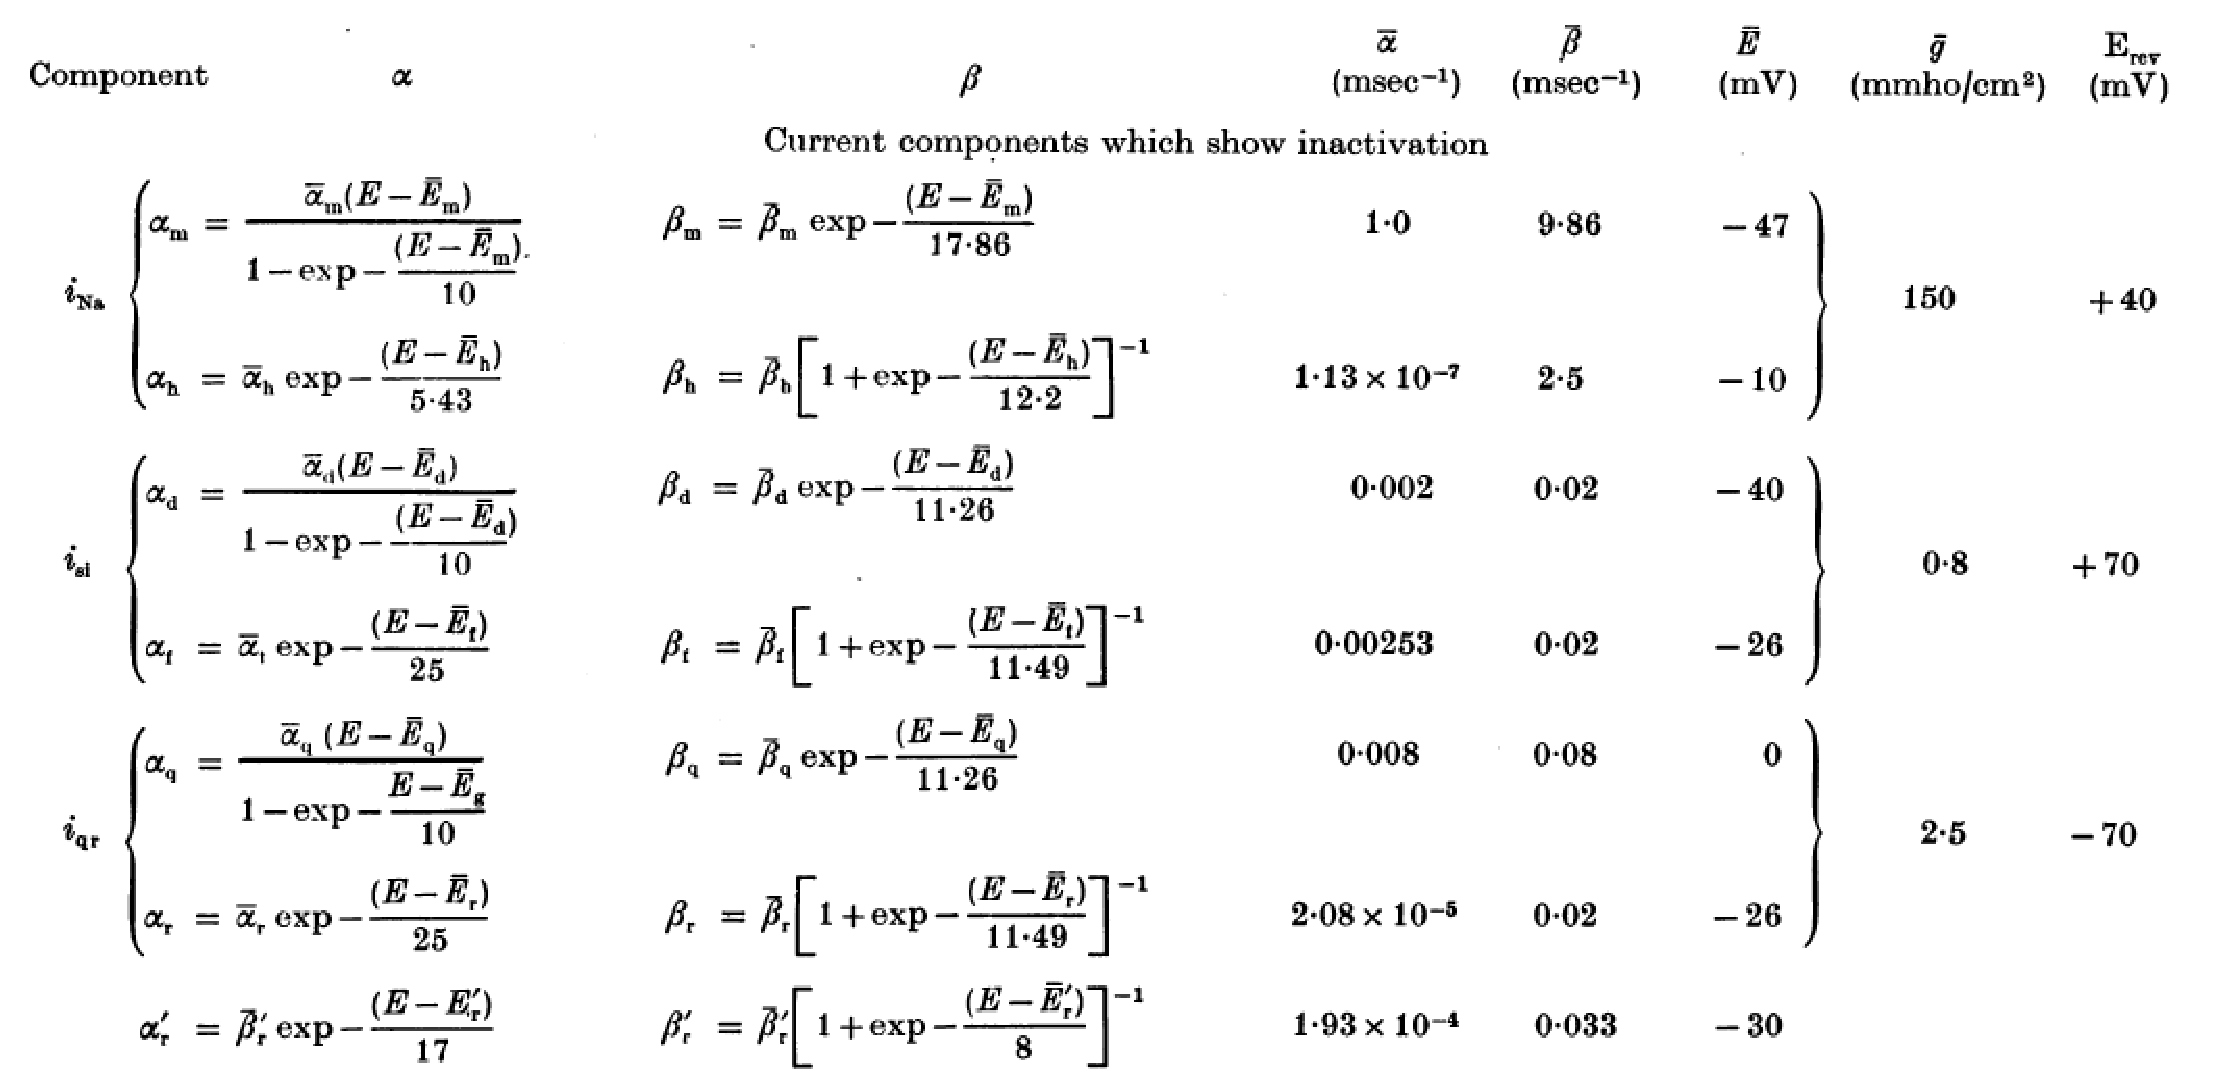
\includegraphics[height=8cm,
    angle=0]{./images/MNT_param.eps}}
  \caption{Parameters setting for gating variables in biphasic ionic
    channels used in MNT model}
\label{fig:MNT_param}
\end{figure}

\begin{figure}[hbt]
  \centerline{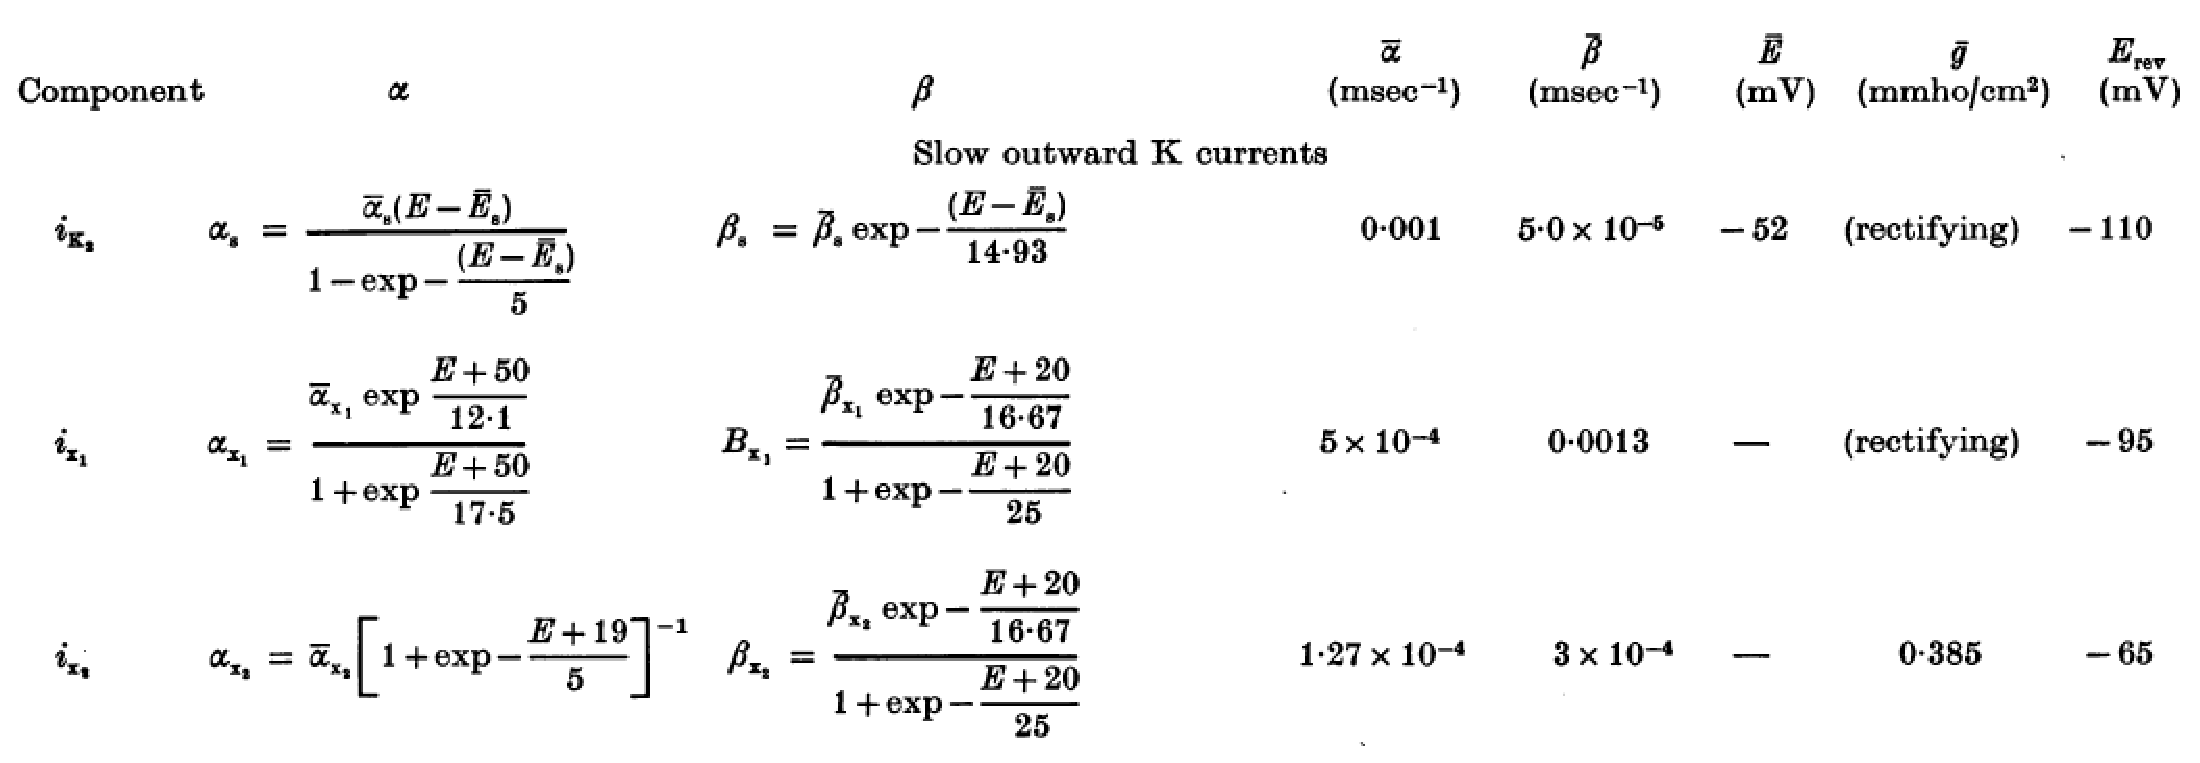
\includegraphics[height=5cm,
    angle=0]{./images/MNT_param2.eps}}
\caption{Parameters setting for gating variables in single phasic
  ionic channels in MNT model}
\label{fig:MNT_param2}
\end{figure}

{\bf IMPORTANT}:
\begin{itemize}
  \item The unit being used in the paper is msec$^{-1}$, while here we use
  sec$^{-1}$.
\item Even though the maximum conductance of individual ion channel is
  not a constant, the total conductance when all channels open is a
  constant, and thus, the average value can be considered as the
  maximum conductance for every channel,
  Fig.~\ref{fig:MNT_out_current}.
\item The measured time constant $\tau$ for a given voltage, e.g. 5-10
  ms near $V_m=0$ mV, is used to detect the parameters for $\alpha,
  \beta$.
\item The half inactivation point $r_\infty$ detected at a given
  voltage, e.g. $r_\infty =1/2$ at $V_m=-80$ mV can also be used to
  detect the parameters for $\alpha, \beta$.
\end{itemize}

\subsection{Analysis}
\label{sec:analysis-7}

Experimental data: \citep{weidmann1955cmp} ($\Na$ current).

Parameter settings:
\begin{itemize}
\item Even though the true capacitance is $\Csc=1\mu$F/cm$^2$, there
  was no available single channel recording, and all was measure w.r.t
  the cylindrical surface area (about 1/10 of the true surface
  area). Thus, the capacitance used for the simulation was $\Csc =
  10\mu$F/cm$^2$. If we want to use $\Csc=1\mu$F/cm$^2$, we should
  divide all ionic currents by 10. 
\end{itemize}

The simulation try to reproduce the result using a short voltage clamp
steps. With this model, it shown a large variability in the frequency
dependence of the notch configuration. For a certain set of
parameters, we can observe a clear notch in every AP, even at high
frequency of stimulus. For other parameter set, the notch appear in
the first AP, and disappear; even at a lower stimulus frequency (see
Fig. 10~\citep{mcallister1975rea}).

\subsection{Summary}
\label{sec:summary-6}

MNT model keep using the assumption ``uniform distribution of ion
channels in surface and in T-tubules''. The model 
\begin{itemize}
\item successfully create
  the notch configuration, separating the spike and the plateau phase of
  an AP. 
\item The AP can occur even there is no rapidly activated Na
  current. 

\item The independence of plateau and pace-maker activity.
\end{itemize}

\section{DiFrancesco-Noble  model (1985)}
\label{sec:difr-noble-purk}

With the availability of single-cell single-channel techniques, there
have been a plethora of experimental data being measured. This
recording technique gave us a more accurate measurement to channel kinetics
which was not available until 1980s. Using this technique, intracellular and
extracellular ion concentrations can be controlled.  Using such
data, and based on previous models, in 1985, DiFrancesco and Noble
developed a new model of Purkinjefiber
AP~\citep{difrancesco1985mcea}.
\begin{itemize}
\item \hyperref[sec:macall-noble-tsien]{M.N.T model} (1975)
\item \hyperref[sec:beeler-reuter-model]{Beeler-Reuter} model (1977)
\item \hyperref[sec:standen_1982model]{Standen-Stanfield model} (1982)
\end{itemize}
The model used the Standen-Stanfield formulation as the basis for the
$\Ca$-dependent inactivation term of $I_\si$; and \textcolor{red}{for the first
time}, ionic pumps are incorporated into a mathematical whole-cell model.

\subsection{Hypothesis analysis}
\label{sec:hypothesis-analysis-1}

There are several changes compared to previous models.

\subsubsection{Ionic currents}

{\bf $I_\Na$}: The new experimental data reveal the new the kinetics of the fast
sodium current $I_\na$ which is quite different from the one in M.N.T
model. Not only permeable to Na, the sodium channel also shown a 12\%
permeability to \ce{K+} ions, eq.~\eqref{eq:713}.

{\bf $I_{\na,b}$}: Along with the change in Na currents, we also need to adjust
the background current, i.e. background sodium current.
The first fact is that the inward background sodium current should be
proportional to the $[Na]_o$. A simple linear relation was assumed. In addition,
it is observed that choline also permeate through this background channels.
Thus, a term for this current $I_{Ch,b}$ was added also, eq.~\eqref{eq:707}.


{\bf $I_{K2} \rightarrow I_f$}: One major change is the re-interpretation of
$I_{K2}$ which change from the (old, incorrect) depolarization-activated inward
K current to the (new, correct) {\bf hyperpolarizing-activated inward K current}
$I_f$ which activates on hyperpolarization negative to -50 mV
~\citep{difrancesco1981nip}. The reversal potential is closed to the $E_K$
(computed in Na-free solution). Experimental data shown that $I_f$ is permeable
to both \ce{Na+} and \ce{K}, as well as increasing external bulk $[K]_b$
increase $I_f$ current. This relation was hypothesized as a simple first-order
binding process - and the binding (if occur) was assumed to be extremely fast,
i.e. the Michaelis-Menten kinetics is utilized, eq.~\eqref{eq:700}
(\textcolor{red}{later results show a sigmoid, not a linear
  relation}).

{\bf $I_\si \rightarrow I_{\ca,f} + I_{\si,2}$}: 
The second inward (or Calcium) current $I_{si}$ was shown to be
permeable to multiple ions, e.g. \ce{K+} can also cross the
channels. Recent experimental results shown that the current is
composed of 2 components: one fast and one slow. The kinetics of the
fast component in $I_{si}$ are very much faster, e.g. at least an
order larger, than $I_{si}$ modeled in M.N.T model and B.R. model,
e.g. activation peak occur within 2-3 ms, and inactivation time
constant lies within 10-20 ms. 
\begin{itemize}
\item The fast component, now denoted as $I_{\ca,f}$ (in guinea-pig
  ventricular cell, frog atrial cell) can permeate both $\Ca$ and $\K$
  with 3 gating variables, as given in eq.~\eqref{eq:717}(a).  If Na
  is taken into account, then an equation similar to
  eq.~\eqref{eq:729}(b) for the Na current can be added.


\item The slow component, which is $[\Ca]_i$-activated component,
  now denoted as $I_{si,2}$ (in mammalian SA node) which can
  corresponds to $I_{Ca,s}$ in the Purkinje fibre. However,
  \textcolor{red}{$I_{\ca,s}$ was not incorporated into the model}.

\end{itemize}

{\bf $I_{x1} + I_{x2} \rightarrow I_{K}$}: The two `plateau'
potassium outward currents $I_{x1},I_{x2}$, now, are combined into a single
{\it time-dependent} potassium current $I_{K}$. This current
shown a simple monotonic function of $[K]_c$, eq.~\eqref{eq:702}

{\bf $I_{K1} \rightarrow I_{K1} + I_{to}$}: In M.N.T. model, the kinetics of the
time-independent background (inward) current $I_{K1}$ was measured by
subtracting all identifiable components. However, exchangers and pumps were not
identified. In that sense, the old $I_{K1}$ indeed contains other unidentified
components. In this model, the exchangers and pumps had been incorporated
explicitly, e.g. Na/K pumps, Na/Ca pumps. As a result, a new interpretation for
``old" $I_{K1}$ is required. Also, with the discovery of a transient
outward-going rectification at potential positive to -20mV, we now have two components
\begin{itemize}
\item $I_{K1}$ is an inward-going background current,
  eq.~\eqref{eq:704}.

\item $I_{to}$ is the transient outward rectifier with
  $[\Ca]_i$-activated and depends on $[K]_b$ (or $[K]_o$ - the bulk or
  external potassium concentration), eq.~\eqref{eq:705}.
\end{itemize}

{\bf $I_\bCa$}: Finally, 
\textcolor{red}{a new component that run in background} to balance the
ionic movements is $I_\bCa$, eq.~\eqref{eq:710}.


\subsubsection{Exchanger (pumps)}
\label{sec:exchanger-pumps}

Now comes the pumps and exchangers. The data from Na/K exchanger show
a stoichiometry ratio 3Na out : 2K in. The net result is one charge
out, thus, there must be an outward current $I_p$ equal to one third
of the net sodium influx generated by the Na/Ca exchange process.  The
Na/K exchanger (pump) was modeled as activated by $[K]_i$ and $[Na]_o$
in eq.~\eqref{eq:708}.

Na/Ca exchanger doesn't consume ATP, so it's assumed that the only
energy available to the process is the gradient of Na and Ca
concentration, and the membrane potential. However, the $V_m$
dependence was unknown. They decided to use the theoretical model
developed by~\citep{mullins1981}. However, it was quite complicated and many
parameters were unknown. Thus, DiFrancesco-Noble used an intermediate
version, eq.~\eqref{eq:712}, which was confirmed with a similar I-V
relation with experimental results~\citep{kimura1986}, and Na:Ca ratio was
chosen with 3:1.

\begin{figure}[hbt]
  \centerline{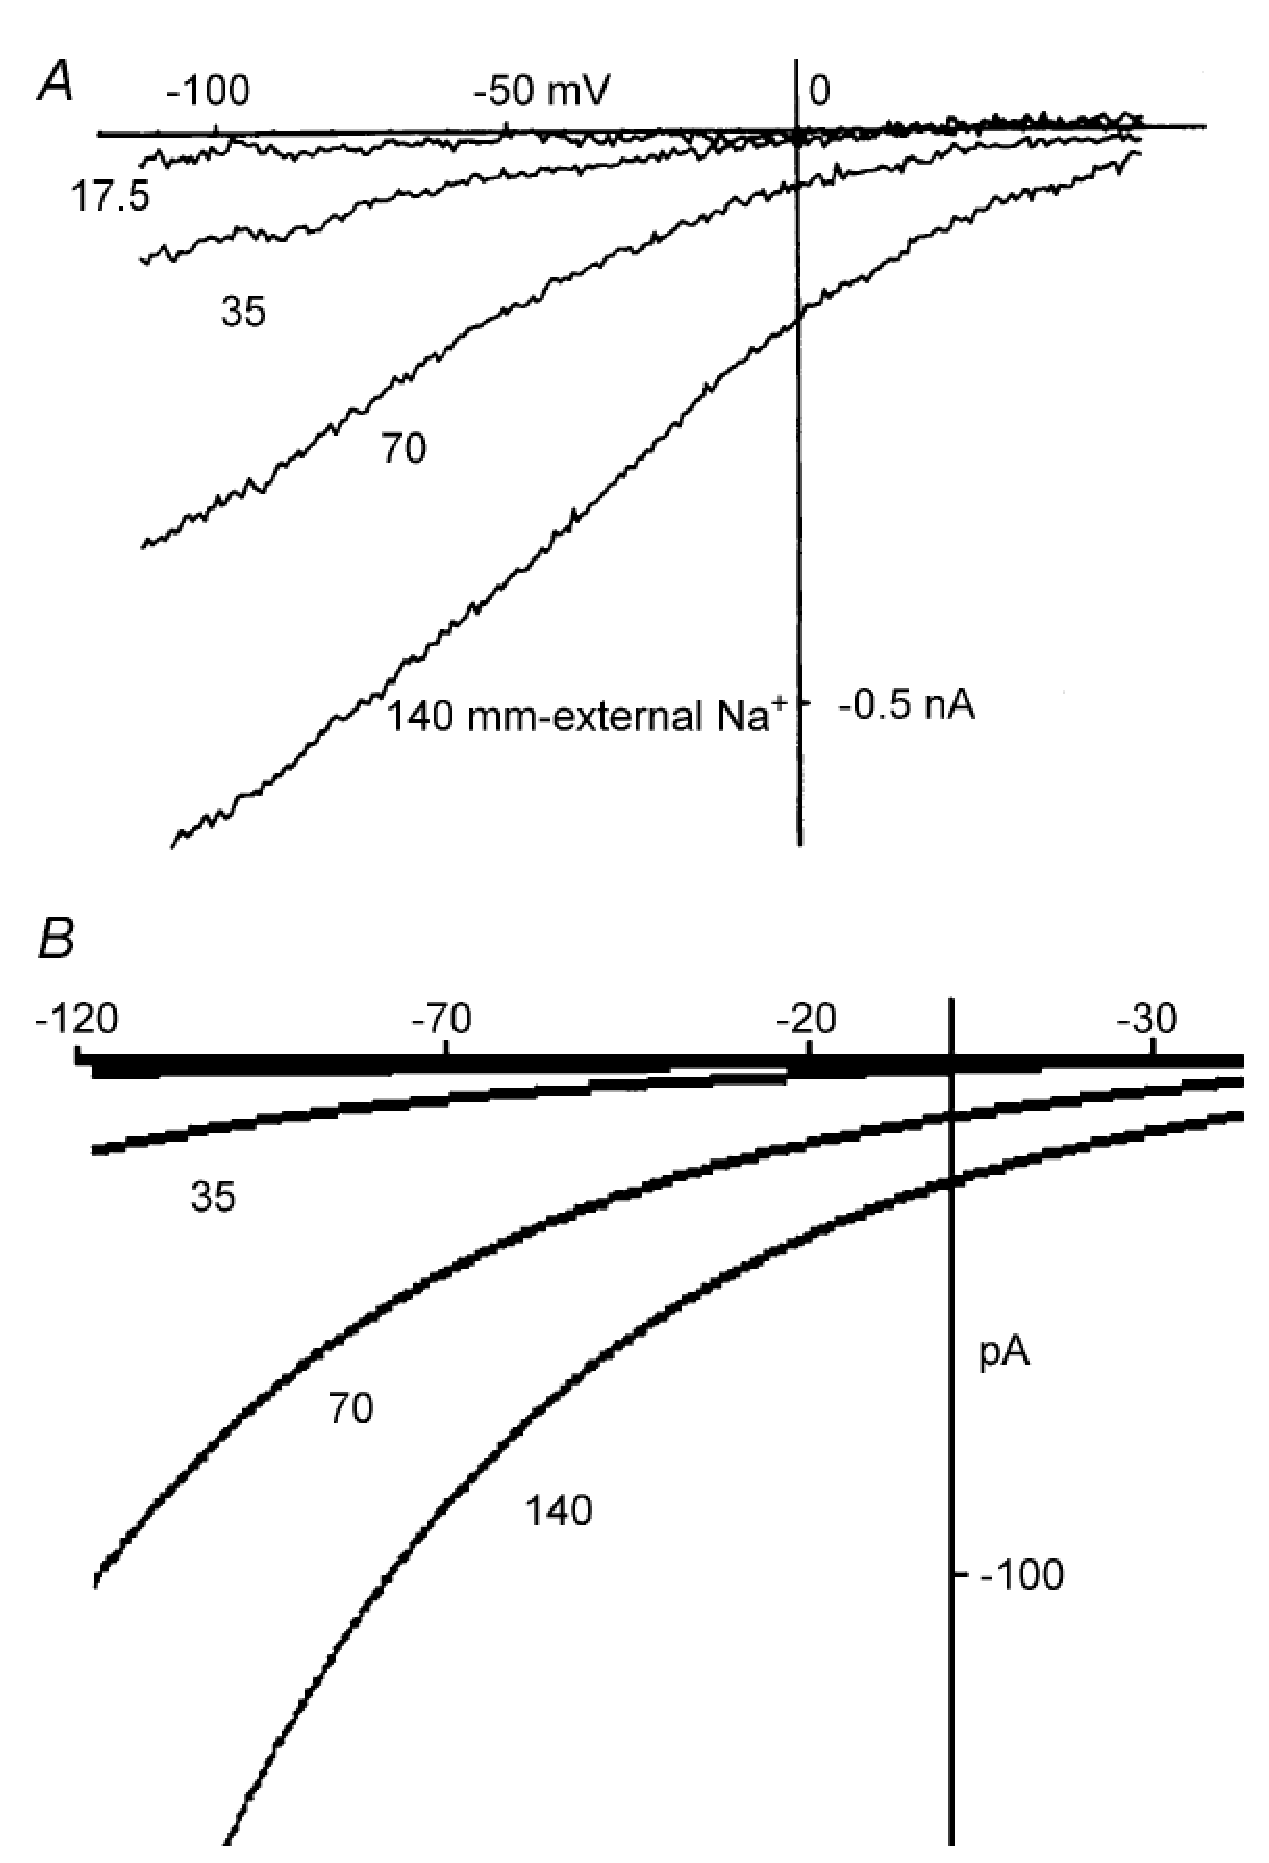
\includegraphics[height=6cm,
    angle=0]{./images/Noble_NaCa.eps}}
  \caption{$I_\NaCa$-V current from experiment (A) and simulation (B)~\citep{noble2007}}
\label{fig:Noble_NaCa}
\end{figure}


% \subsubsection{Ion Concentration}
% \label{sec:concentration-1}
% 

\subsection{Mathematical model}
\label{sec:mathematical-model-9}

\textcolor{red}{The voltage is in [mV]. The conductances are measured
  at whole-cell level, so $g_i$ is in unit of $\mu$S. Correspondingly,
  all currents' units are (nA)}.

\begin{enumerate}


\item Based on the fact that Na channels also allow 12\% of \ce{K+} ion to
permeate, the equation was
  \begin{equation}
    \label{eq:713}
      I_{\na} =g_{\na} m^3h (V_m-E_{mh}) 
  \end{equation}
  with $g_{\na}=750\mu$S to generate the maximum depolarization rate.
  $E_{mh}$ is the Nernst reversal potential.
  \begin{equation}
    \label{eq:748}
    E_{mh} = \frac{RT}{F} \ln\left[\frac{[Na]_o+PR_{NaK}[K]_c}{[Na]_i+PR_{NaK}[K]_i}\right]
  \end{equation}
  with $PR_{NaK}=0.12$ is the Na/K permeability ratio. 

  The two gating variables follow first-order kinetics
  \begin{equation}
    \label{eq:714}
    \begin{split}
      \frac{dm}{dt} &= \alpha_m(1-m)-\beta_m.m \\
      \alpha_m &= 200\frac{(V_m+41)}{1-\exp(0.1(V_m+41))}\;;
      (\alpha_m = 2000, \text{ when } V_m=-41) \\
      \beta_m &= 8000\exp(-0.056(V_m+66)) \\
      \frac{dh}{dt} &= \alpha_h(1-h)-\beta_h.h \\
      \alpha_h &= 20\exp(-0.125(V_m+75)) \\
      \beta_h &= \frac{2000}{320.\exp(-0.1(V_m+75))}
    \end{split}
  \end{equation}
  The kinetics of $m$ was similar to that of Hodgkin-Huxley model,
  except it was shifted to obtain the steady-state value of 0.5 at
  $V_m=-30$ mV (fit to experimental data). The kinetics of $h$ was
  fitted to experimental data to give $h_\infty=0.5$ at $V_m=-70$
  mV. The rate constant was adjusted to give  $\tau_h=50$ ms at
  $V_m=-80$ mV, decreasing to 0.7 ms at $V_m=0$ mV. 

\item The hyperpolarizing-activated inward K current $I_f$
  \begin{equation}
    \label{eq:700}
    I_f = \frac{[K]_c}{[K]_c+K_{m,t}} (g_{f,K}+g_{f,Na}).y
  \end{equation}
  with $g_{f,K}=3\mu$S, $g_{f,Ka}=3\mu$S. $K_{m,f}$ is the value of
  $[K]_b$ for half-activation; $[K]_c$ is the potassium concentration
  in the cleft. The gating variable $y$ 
  \begin{equation}
    \label{eq:701}
    \begin{split}
      \frac{dy}{dt} &= \alpha_y(1-y)-\beta_y.y \\
      \alpha_y &= 0.025 \exp(-0.067\times (V_m+52))\\
    \end{split}
  \end{equation}
  \begin{equation*}
    \left[ \begin{array}{l}
        \beta_y = \frac{0.5(V_m+52)}{1-\exp[0.2(V_m+52)]}\\
        (\beta_y)_{V_m=-52}=2.5
        \end{array}\right.
  \end{equation*}
\item Second inward current formula can permeate both $\Ca$ and $\K$,

  \begin{equation}
    \label{eq:717}
    I_{Ca,f} = d\times f\times f_2\times(I_{si,Ca}+I_{si,K}) 
  \end{equation}
  in which the component current for each ions is modeled using a
  constant field type formulation for the individual ion movements
  \begin{equation}
    \label{eq:729}
    \begin{split}
      I_{si,Ca} &=
      P_{si}\frac{z_\ca^2
        F^2}{RT}\frac{V_m-50}{1-\exp(-(V_m-50)z_\ca F/RT)}
      \times \\
      &([\Ca]_i \exp(\frac{V^\theta F}{RT}) -
      [\Ca]_o\exp(-(V_m-50)\frac{z_\ca F}{RT})) \\
      I_{si,K} &= 0.01P_{si}
      \frac{(V_m-50)(z_\k^2 F^2/(RT))}{1-\exp(-(V_m-50)F/RT)}\times \\
      &([K]_i\exp(50F/(RT))-[K]_c \exp(-(V_m-50)F/(RT)))
    \end{split}
  \end{equation}
  with $V^\theta=100$mV, $z_\k=1, z_\ca=2$. $P_\si$ is the
  permeability of $\Ca$ ions via the channel. The permeability of $\K$
  is a hundred time smaller, so that we use $0.01 P_\si$.

  The kinetics is modelled as Voltage-dependent activation $d$; and
  Voltage-dependent inactivation $f$, and Calcium-dependent
  inactivation $f_2$.  Compared to B.R. model, the time constant for
  the gating variables in Purkinje fibre are faster (2-5 ms for
  activation and 10-20 ms for inactivation).
  \begin{equation}
    \label{eq:384}
    \begin{split}
      \frac{dd}{dt} &= \alpha_d(1-d)-\beta_d d \\
      \alpha_d &= \frac{30(V_m+24)}{1-\exp[-\frac{V_m+24}{4}]}\\
      \text{NOTE: } \alpha_d|_{V_m=-24}&=120 \\
      \beta_d &= \frac{12(V_m+24)}{-1 + \exp[\frac{V_m+24}{10}]} \\
      \text{NOTE: } \beta_d|_{V_m=-24} &= 120
    \end{split}
  \end{equation}
  These values were chosen to give a half-maximal of the current
  $I_{\ca,f}$ at -34 mV, and a peak time constant of about 20ms. This
  produces $I_{si,Ca}$ peak in less than 5ms and is largely inactivated
  by 50 ms. For the Ca-dependent inactivation, $f_2$ is derived from
  Standen-Stanfield formula (1982).
  \begin{equation}
    \label{eq:730}
    \frac{df_2}{dt} = \beta_{f_2}.(1-f_2) - \alpha_{f_2} . f_2 [\Ca]_i
  \end{equation}
At steady-state, the degree of inactivation $(1-f_2)$ is given by
\begin{equation}
  \label{eq:731}
  1-f_2 = \frac{[\Ca]_i}{[\Ca]_i+K_{m,f_2}}
\end{equation}
where $K_{m,f_2}=\frac{\alpha_{f_2}}{\beta_{f_2}}$. The chosen value
$K_{m,f_2}=1$mM gives negligible inactivation at resting potential of
$[\Ca]_i$, yet appreciable inactivation during $[\Ca]_i$ transient. 

\item The delayed \ce{K+} current
  \begin{equation}
    \label{eq:702}
    I_{K} = I_{K,max}\frac{[K]_i-[K]_c\exp(-\frac{V_m}{25})}{140}.x
  \end{equation}
  The gating variable $x$ is
\begin{equation}
  \label{eq:703}
  \begin{split}
    \frac{dx}{dt} &= \alpha_x(1-x)-\beta_x.x \\
    \alpha_x &= 0.5 \frac{\exp(0.0826\times (V_m+5))}{}\\
    \beta_x &= 1.3\frac{\exp(-0.06(V_m+20))}{1+\exp(-0.04(V_m+20))}
  \end{split}
\end{equation}

NOTE: In earlier models, the usual maximum outward current $I_\k$ at
positive potentials when $[K]_i=140$nM is 180nA; thus $[K]_i$ is
usually set to 140nM.


\item The time-independent background outward \ce{K+} current
  $I_{\k1}$ was based on Hagiwara-Takahashi equation(1974) - an
  empirical equation and quite simpler than that of
  Hille-Schwarz(1978)
  \begin{equation}
    \label{eq:704}
    I_{K1} =
    \overline{g_{K1}}
    \frac{[K]_c}{[K]_c+K_{m,1}}
    \frac{V_m-E_K}{1+\exp[\frac{z_\ca F}{RT}(V_m-E_K+10)]}   
  \end{equation}
  The binding of \ce{K+} to the channel was assumed to be
  instantaneous. Thus, Michaelis-Menten can be applied with a
  calculated binding constant of $K_{m,1}=210$mM (at $V_m=-100$mV),
  and maximum conductance (during strong hyperpolarization)
  $\overline{g_{K1}}=920\mu$S. 
  
  NOTE: \textcolor{red}{Sakman and Trube~\citep{sakmann1984cps} also figured out
  that the channel also have others substates of conductance, yet the model did
  not considered this}.

\item The transient outward current 
  \begin{equation}
    \label{eq:705}
    \begin{split}
      I_{to} =
      0.28\frac{0.2+[K]_c}{K_{m,1}+[K]_c}\times \frac{[\Ca]_i}{K_{m,to}+[\Ca]_i}
      \times\frac{V_m+10}{1-\exp[-0.2(V_m+10)]}\\
      \times\left( [K]_i\exp(0.02V_m)-[K]_o\exp(-0.02V_m) \right)
      \times r
    \end{split}
  \end{equation}
  \begin{itemize}
  \item The first term represent the activation by external cleft-space $[K]_c$
    which saturate at about $30$mM. The equilibrium constant
    $K_{m,1}=210$ mM (similar to above)
 
  \item The second term is $[\Ca]_i$ activation. The equilibrium
    constant $K_{m,to}=1\mu$M to allow normal $[\Ca]_i$ transient to activate
    the current with correct magnitude~\citep{segelbaum1980cto}.
  \item The third term represent $V_m$-dependent, which was set to 5
    when $V_m=-10$ to avoid zero in the denominator.
  \item The final term is obtained from the {\it rate theory}
  (Sect.\ref{sec:eyring-rate-theory}) assuming that the energy barrier is placed
  at the center of the membrane
  \end{itemize}
  The gating (inactivation) variable $r$ follow the first-order kinetics
\begin{equation}
  \label{eq:706}
  \begin{split}
    \frac{dr}{dt} &= \alpha_r(1-r)-\beta_r.r \\
    \alpha_r &= 0.033\exp(-V_m/17)\\
    \beta_r &= \frac{33}{1+\exp(-\frac{V_m+10}{8})} \\
  \end{split}
\end{equation}

\item The inward background sodium current 
  \begin{equation}
    \label{eq:707}
    I_{\na,b} = \frac{[Na]_o}{[Na]_{o,c}}g_{\na,b}(V_m-E_{\na})+I_{\Ch,b}
  \end{equation}
with $g_{\na,b}=0.18\mu$S. $[Na]_{o,c}=140$mM is the control level of $[Na]_o$

\item The resting background calcium leak
  \begin{equation}
    \label{eq:710}
    I_\bCa = g_\bCa (V_m-E_{Ca})
  \end{equation}
with $g_\bCa=0.02\mu$S to keep the resting calcium $[\Ca]_i$ in the
range 0.05-0.1$\mu$M. 

\end{enumerate}

{\bf Exchanger (pumps)}
\begin{enumerate}
\item The Na/K exchanger (3Na out : 2K in)
  \begin{equation}
    \label{eq:708}
    I_p = \overline{I_p} \frac{[K]_c}{K_{m,K}+[K]_c} \times 
    \frac{[Na]_i}{K_{m,Na}+[Na]_i}
  \end{equation}
  The exchanger was assumed to be activated by extracellular cleft $[K]_c$
  and cytoplasmic $[Na]_i$ as first-order and fitted by
  Michaelis-Menten kinetics. The two equilibrium constants (for
  half-activation) of $[K]_c$ and $[Na]_i$ are $K_{m,K}=1$mM,
  $K_{m,Na}=40$mM. $\overline{I_p}=125$nA (maximum current), respectively.

  NOTE: Different groups obtained different values for $K_{m,K}$. This
  was explained by the restricted extracellular space used by
  different experiments. Thus, with the assumption of extracellular
  space to be largest, the smallest $K_{m,K}$ was chosen,
  i.e. $K_{m,K}= 1$mM, the value obtained by Gadsby (1980).  The
  maximum current is about 20nA when $[K]_c=4$mM, $[Na]_i=9$mM.

\item The Na/Ca exchanger (NCX) was a simplified version
  of~\citep{mullins1977mnc}
  \begin{equation}
    \label{eq:712}
    \begin{split}
      I_\NCX =
      k_\NCX\exp\left(\frac{\gamma(n_\NCX-2)EF}{2RT}[Na]_i^n[\Ca]_o\right) \\
      -\frac{\exp(-(1-\gamma)(n_\NCX-2)EF/(2RT))[Na]_i^n[\Ca]_o}{1+d_\NCX([\Ca]_i[Na]_o^n
        + [\Ca]_o[Na]_i^n)}
    \end{split}
  \end{equation}
  In Mullins formulation, the constant 1 in the denominator is
  substituted by a function of sodium concentration, to take proper
  account of $[Na]_i$ and $[Na]_o$ changes. In the standard model,
  $\gamma=0.5$, i.e. the position of the energy barrier is the center
  of the membrane (read the rate theory). A suitable value for
  $k_\NCX=.02$ and $d_\NCX=0.001$.

  Some of the variables in eq.~\eqref{eq:712} are fixed,
  e.g. $[Na]_o=140$mM, $[\Ca]_o = 2$mM; or can be computed from the
  model, e.g. $[\Ca]_i, [Na]_i$. 

\end{enumerate}

{\bf Ion concentrations}: 

\begin{enumerate}
\item Extracellular K concentration (in the cleft space): assume to
  diffuse freely be constant. For a cylinder preparation, we use
  \begin{equation}
    \label{eq:715}
    \begin{split}
      \frac{\partial [K]_c}{\partial t} = D\left[
        \frac{\partial^2[K]_c}{\partial x^2} + \frac{1}{x} \frac{\partial
          [K]_c}{\partial x}\right] + \frac{I_{m,K}}{V_eF} \\
      I_{m,K} = I_{K1} + I_{K} + I_{f,K} + I_{si,K} + I_{K,b} - 2I_p
    \end{split}
  \end{equation}
  with $V_e$ is the extracellular space volume. For a cylinder, we
  have
  \begin{equation}
    \label{eq:733}
    V_e = V_{ecs}a^2l 
  \end{equation}
with $V_{ecs}$ is the fraction extracellular space (usually set up to
5\%), $a$ is the radius and $l$ is the length of the cylinder. 


For a sphere preparation, we use
\begin{equation}
  \label{eq:735}
    \frac{\partial [K]_c}{\partial t} = D\left[
      \frac{\partial^2[K]_c}{\partial x^2} + \frac{2}{x} \frac{\partial
        [K]_c}{\partial x}\right] + \frac{I_{m,K}}{V_eF} 
\end{equation}
\item Intracellular K concentration
  \begin{equation}
    \label{eq:716}
    \frac{d[K]_i}{dt} = \frac{I_{m,K}}{V_i.F}
  \end{equation}
with $V_i$ is the volume of the intracellular fluid.

\item Intracellular Na concentration (under the assumption of
  negligible binding of Na, i.e. no buffering)
  \begin{equation}
    \label{eq:732}
    \frac{d[Na]_i}{dt} = -\frac{I_{Na}+I_{Na,b}+I_{Na,f}+I_{si,Na}+3I_p+(\frac{n_\NCX}{n_\NCX-2})I_\NCX}{V_iF}
  \end{equation}
with $V_i$ is the volume of the intracellular fluid.
\begin{equation}
  \label{eq:734}
  V_i = (1-E_{ecs})V_e
\end{equation}


\item Intracellular $[\Ca]_i$.  This is complex as Ca buffering is
  important, yet not very well understood. 
\begin{figure}[hbt]
  \centerline{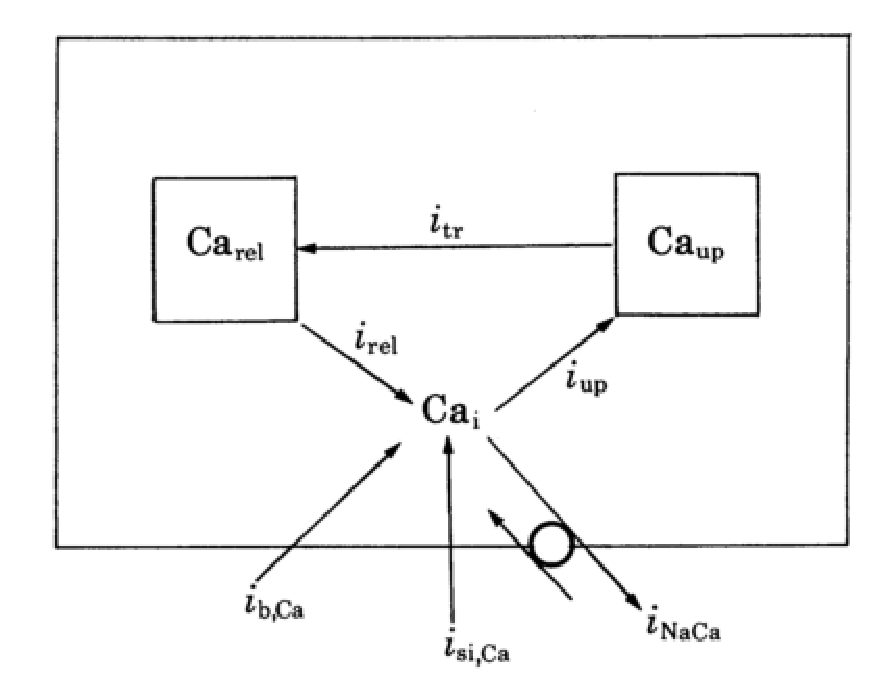
\includegraphics[height=5cm,
    angle=0]{./images/DN_calcium_sequest.eps}}
  \caption{Hypothesized process of calcium movement within cells and
    across the cell membrane: An energy-consuming pump is assumed to
    transport Ca back to the SR ($I_{up}$), then Ca release is
    activated by $[\Ca]_i$. Ca enters the cell through background leak
    and ($I_\bCa$) and gated channel ($I_{si,Ca}$) - rarely it can
    enter the cell via Na-Ca exchanger, only when $[\Ca]_i$ is very low
    and potential is very positive. Ca leaves the cell via Na-Ca
    exchange. Other possible process that haven't been considered like
    Voltage-dependent Ca release, Ca-ATP pumps, other calcium
    sequestering process}
\label{fig:DN_calcium}
\end{figure}

It is assumed that the major calcium sequestration (uptake store) is
the network SR, and SR occupies 5\% of the intracellular fluid volume
($V_{up}=0.05V_i$), and can sequester up to 5 mM \ce{Ca^2+},
i.e. $[\overline{Ca}]_{up}=5$ mM (Chapman (1979)). A fraction of Ca from
the uptake store then can be transferred ($I_{tr}$) to a separate
release store $[\Ca]_{rel}$\footnote{later know as the junctional SR}
which then can be converted ($I_{rel}$) to a releasable form
$Ca_{i}$. The $I_{tr}$ process can be $V_m$ dependent, thus we need a
gating variable $p$. The $I_{rel}$ process is induced by Calcium,
i.e. CICR, with the requirement of $r$ calcium
bindings~\citep{fabiato1975cic}.
\begin{equation}
  \label{eq:737}
  \begin{split}
    \frac{d[\Ca]_{up}}{dt} &= \frac{I_{up}-I_{tr}}{2V_{up}F} \\
\frac{d[\Ca]_{rel}}{dt} &= \frac{I_{tr}-I_{rel}}{2V_{rel}F} \\
\frac{d[\Ca]_i}{dt} &= -\frac{I_{si,Ca}+I_{b,Ca} -
  \frac{2I_\NCX}{n_\NCX-2} + I_{up} - I_{rel}}{2V_iF}
  \end{split}
\end{equation}
where $V_{up}, V_{rel}$ are the volumes of the uptake and release
stores respectively. Using the data from ventricular
muscle~\citep{chapman1979} where it is assumed that
$V_{up}=0.05V_i$. $V_\rel=0.02V_i$. 

The associated currents are
\begin{equation}
  \label{eq:738}
  \begin{split}
    I_{up} = \alpha_{up}[\Ca]_i ([\overline{Ca}]_{up} - [\Ca]_{up}) -
    \beta_{up}[\Ca]_{up} \\
    I_{tr} = \alpha_{tr}p([\Ca]_{up}-[\Ca]_{rel}) \\
    I_{rel} = \alpha_{rel}[\Ca]_{rel}\frac{[\Ca]_i^r}{[\Ca]_i^r + K_{m,Ca}}
  \end{split}
\end{equation}
with $\overline{[\ca]}_{up}=5$ mM ($\Ca$ sequestering capability of SERCA
pump measured by~\citep{chapman1979}), with $r$ is the number of
\ce{Ca^2+} ions assumed to bind to the release site ($r=1$ or
$2$). $K_{m,ca}=0.001$ mM when $r=1$, and 0.001$^2$ mM when $r=2$.
\begin{equation}
  \label{eq:739}
  \frac{dp}{dt} = \alpha_p(1-p)-\beta_p p
\end{equation}
is the time- and $V_m$-dependent of the exchange between storage and
release sites. The gating variables were chosen the same as those of
$f$, yet slowed by a factor of 10.

\begin{equation}
  \label{eq:1350}
  \begin{split}
    \alpha_\up &= \frac{z_\ca FV_i}{\tau_\up \overline{[\ca]}_\up} \\
    \alpha_\tr &=  \frac{z_\ca FV_i}{\tau_\tr} \\
    \alpha_\rel &=  \frac{z_\ca FV_i}{\tau_\rel} \
  \end{split}
\end{equation}
with the time constants were chosen $\tau_\rel=50$ ms to enable
$[\Ca]_i$ to reach the peak within 50 to 100ms, repriming time
constant $\tau_{rep}$ was set to 2ms at -80 mV. The uptake time
constant $\tau_\up =25$ ms to allow the uptake to occur significantly
rapid to reproduce the falling phase of $[\Ca]_i$ transient. 

\end{enumerate}

\subsection{Analysis}
\label{sec:analysis-9}

\begin{figure}[hbt]
  \centerline{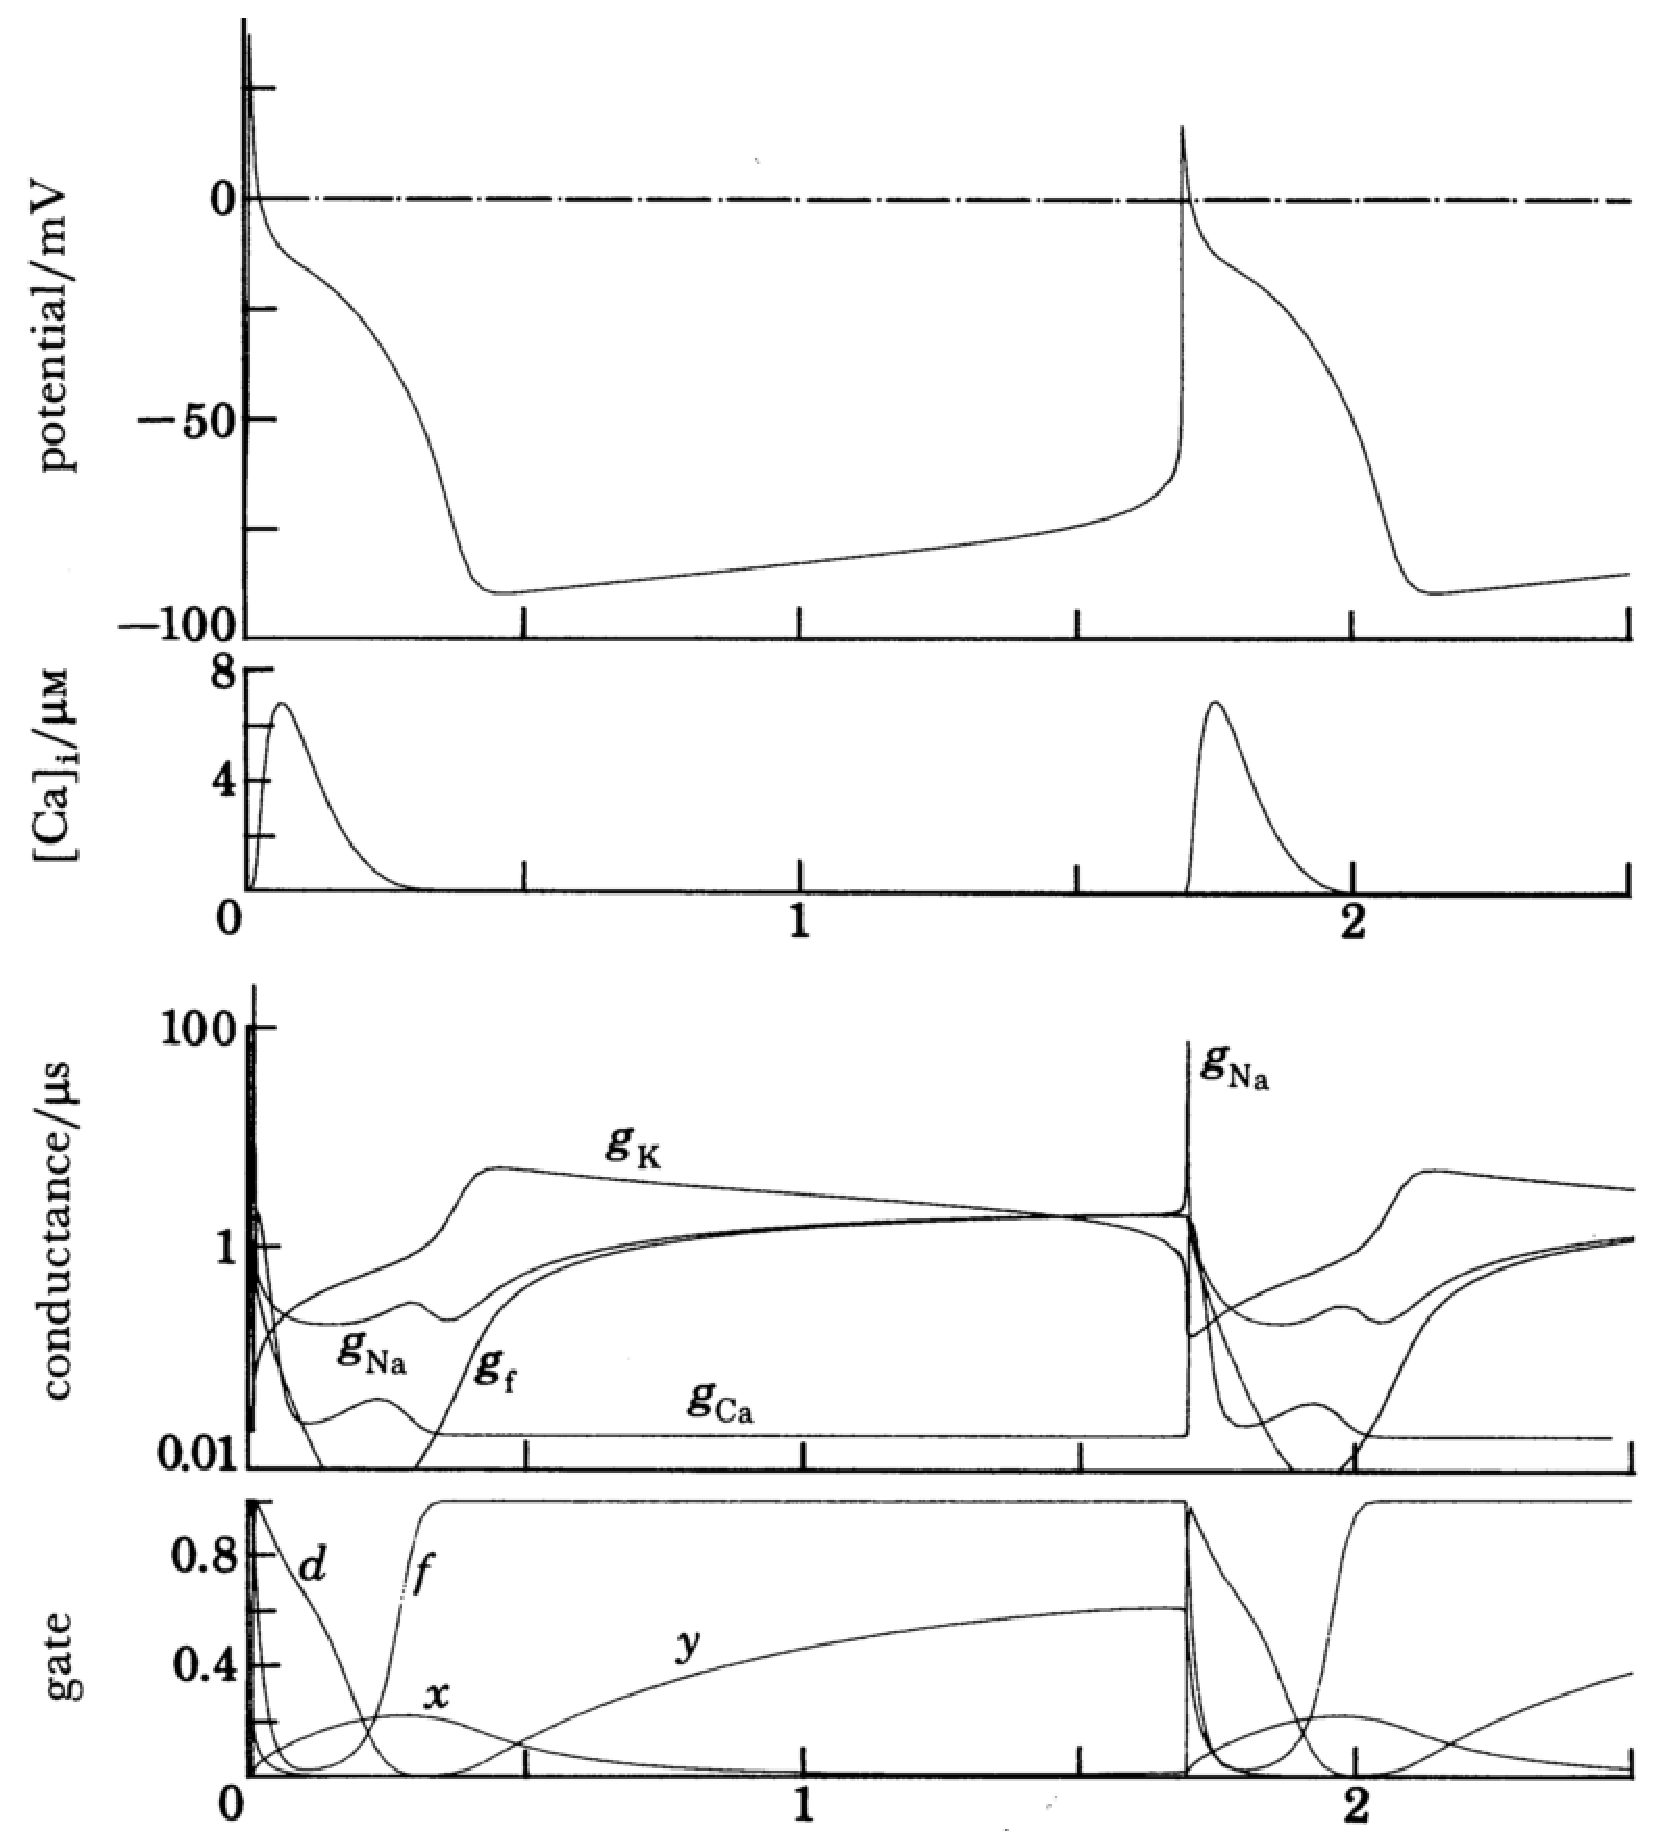
\includegraphics[height=7cm,
    angle=0]{./images/DiFrancesco_purkinjie.eps}}
  \caption{standard AP, $[\Ca]_i$ transient, conductances (on
    logarithmic scale), and gating variables computed for
    external bulk $[\k]_b=4$mM}
\label{fig:DiFrancesco_purkinje}
\end{figure}

\textcolor{blue}{DiFrancesco-Noble model has 9 currents (ionic channes
  + exchanger) and took into account the change of 4 ionic
  concentrations}.
For the first time, we have a whole-cell model fully integrates the
electrophysiological description of gated channels in the heart with a
description of ionic pumps and sequestering process. However, the
model has not taken into account buffering of $\ca$.

\begin{figure}[hbt]
  \centerline{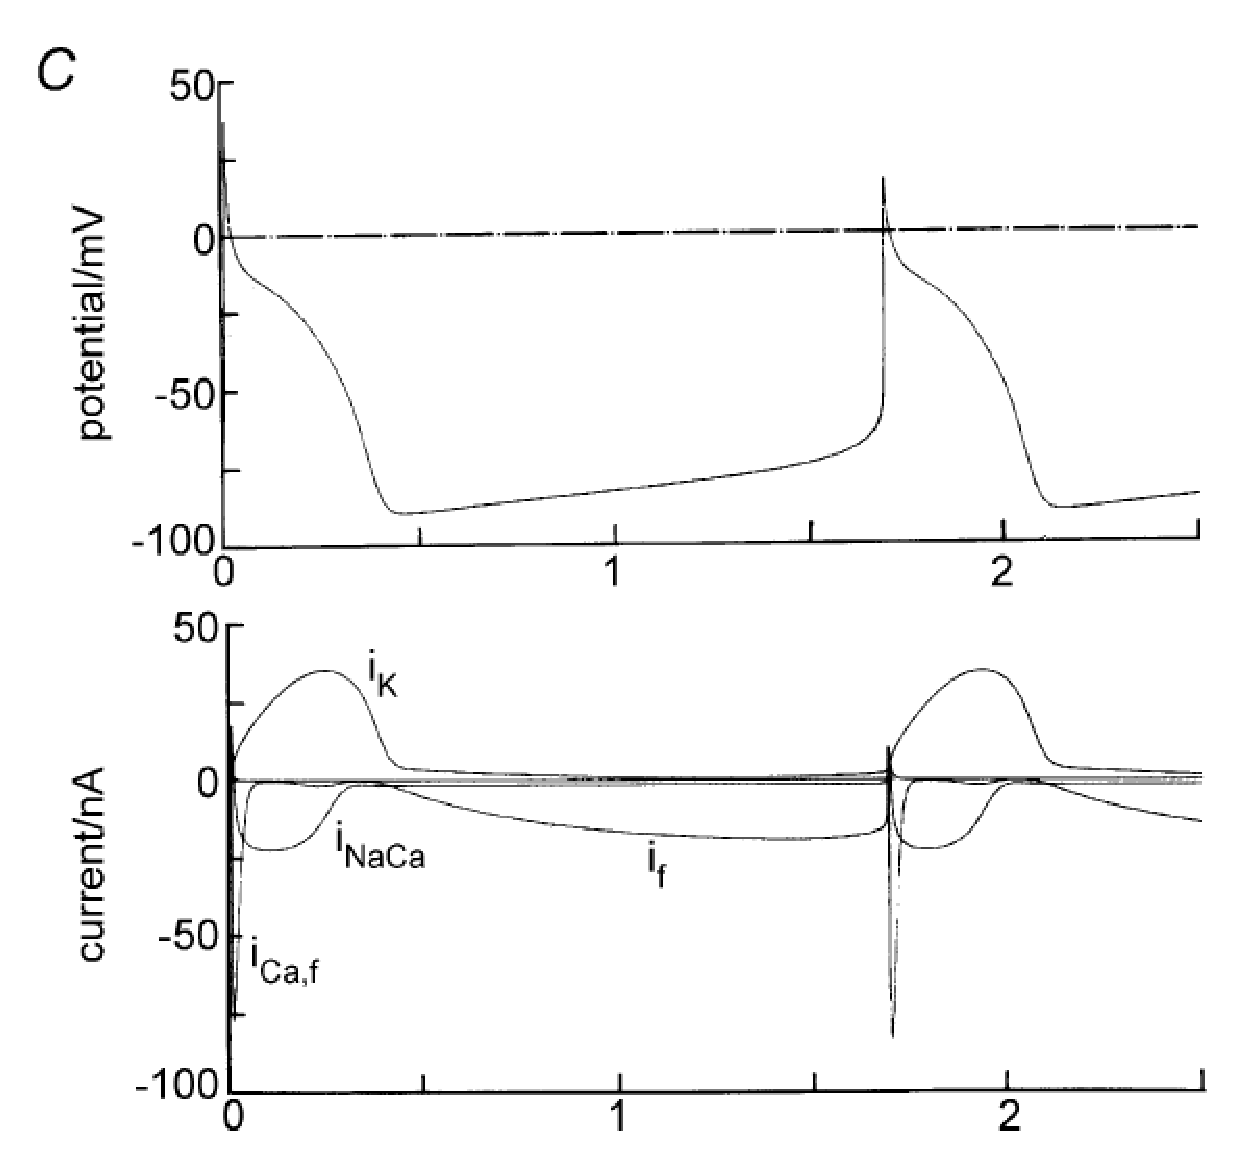
\includegraphics[height=7cm,
    angle=0]{./images/Noble_purkinje.eps}}
\caption{Ionic components contributing during AP}
\label{fig:Noble_purkinjee}
\end{figure}

The background Na is carried by non-specific channels (as it allow
both Na and K). 

Compared to the Na/Ca exchanger model by ~\citep{mullins1977mnc}, this model
only consider Ca-dependence and remove Na-dependence. Thus, the Na-dependence
term was replaced by a constant term.

In a 3-compartment model, we have the bulk $[\K]_b$, the cleft space $[\K]_c$
and the intracellular space $[\K]_i$. Thus, if $P$ is the rate constant for
exchange between the bulk and cleft space ($P$ between 0.2 and 1.0$s^{-1}$), we
have
\begin{equation}
  \label{eq:736}
  \frac{d[K]_c}{dt} = -P([K]_c - [K]_b) + \frac{I_{m,k}}{V_iF}
\end{equation}


By changing $[K]_c$, we collect the following results for analysis
(Fig.6,7.8)
\begin{itemize}
\item AP: shorten in duration and suppression pacemaker activity
  (degraded) at high $[K]_b$
\item increase automaticity  at moderately low $[K]_b$, e.g. $[K]_b=4$ mM.
\end{itemize}

\section{Hirano-Fozzard-January (1989)}

\citep{hirano1989}

\section{Tseng-Boyden (1989)}

\citep{tseng1989} 

\section{Li-Rudy (2011) - canine}

Under the same condition, it has been suggested that Pcell is more vulnerable to
DAD and arrhythmic activity than ventricular cell (Vcell), e.g. CPVT and
ventricular fibrillation. Even though Purkinje cells (Pcell) are frequently
involved in ventricular arrhythmias, the mechanistic basis for their arrhythmic
vulnerability is not well understood. 

Pcell has a faster depolarization upstroke, and sloping repolarization time
course during phase two, and longer APD. Also, Pcell doesn't have the T-tubular
network. Pcell exhibits biphasic $\Ca$ transients (CaT) in response to normal
membrane depolarization. Pcell has a complex, triple-layer spatial distribution
of RyR2, RyR3 and IP3R. 

\citep{li2011} developed a new compartmental model (PRd model) of canine cardiac
Purkinje AP.

\subsection{Model development}

The data is measured at 37$^\circ$C.  The model is represented as a cylinder 164
$\mum$ in length, 17.5$\mum$ in radius. The SR is divided into 3 compartments:
junctional SR (jSR), corbular SR (cSR) and network SR (nSR). The cytoplasm is
divided into 3 regions: peripheral coupling subspace (PCS), subsarcolemmal
region (SSL) and bulk myoplasm. PCS is equivalent to the dyad in the ventricular
myocyte. Howeve, the term dyad is not applied in Pcell as it lacks the T-tubular
network. The SSL is the region underneath the sarcolemmal membrane of 2$\mum$
deep. There is a 'void' region (2$\mum$) between SSL and bulk myoplasm, with
virtually no expression of RyR2 and IP3R, and with reduced RyR3 compared to SSL.
All ionic currents, not in PCS, are on SSL.


\subsection{Data analysis}

Membrane resting potential is -84.6 (mV). During steady-state pacing (BCL =
500ms), APD90 = 293.2ms; maximum upstroke velocity of 461 V/sec.

Simulated drug effects (TTX, nifedipine, TEA) on Pcell AP morphology are
consistent with experimental data. The {\bf adaptation curve} is the plot BCL
vs. APD90. 

%%% Local Variables: 
%%% mode: latex
%%% TeX-master: "mainfile"
%%% End: 
